\documentclass[twoside]{book}

% Packages required by doxygen
\usepackage{fixltx2e}
\usepackage{calc}
\usepackage{doxygen}
\usepackage[export]{adjustbox} % also loads graphicx
\usepackage{graphicx}
\usepackage[utf8]{inputenc}
\usepackage{makeidx}
\usepackage{multicol}
\usepackage{multirow}
\PassOptionsToPackage{warn}{textcomp}
\usepackage{textcomp}
\usepackage[nointegrals]{wasysym}
\usepackage[table]{xcolor}

% Font selection
\usepackage[T1]{fontenc}
\usepackage[scaled=.90]{helvet}
\usepackage{courier}
\usepackage{amssymb}
\usepackage{sectsty}
\renewcommand{\familydefault}{\sfdefault}
\allsectionsfont{%
  \fontseries{bc}\selectfont%
  \color{darkgray}%
}
\renewcommand{\DoxyLabelFont}{%
  \fontseries{bc}\selectfont%
  \color{darkgray}%
}
\newcommand{\+}{\discretionary{\mbox{\scriptsize$\hookleftarrow$}}{}{}}

% Page & text layout
\usepackage{geometry}
\geometry{%
  a4paper,%
  top=2.5cm,%
  bottom=2.5cm,%
  left=2.5cm,%
  right=2.5cm%
}
\tolerance=750
\hfuzz=15pt
\hbadness=750
\setlength{\emergencystretch}{15pt}
\setlength{\parindent}{0cm}
\setlength{\parskip}{3ex plus 2ex minus 2ex}
\makeatletter
\renewcommand{\paragraph}{%
  \@startsection{paragraph}{4}{0ex}{-1.0ex}{1.0ex}{%
    \normalfont\normalsize\bfseries\SS@parafont%
  }%
}
\renewcommand{\subparagraph}{%
  \@startsection{subparagraph}{5}{0ex}{-1.0ex}{1.0ex}{%
    \normalfont\normalsize\bfseries\SS@subparafont%
  }%
}
\makeatother

% Headers & footers
\usepackage{fancyhdr}
\pagestyle{fancyplain}
\fancyhead[LE]{\fancyplain{}{\bfseries\thepage}}
\fancyhead[CE]{\fancyplain{}{}}
\fancyhead[RE]{\fancyplain{}{\bfseries\leftmark}}
\fancyhead[LO]{\fancyplain{}{\bfseries\rightmark}}
\fancyhead[CO]{\fancyplain{}{}}
\fancyhead[RO]{\fancyplain{}{\bfseries\thepage}}
\fancyfoot[LE]{\fancyplain{}{}}
\fancyfoot[CE]{\fancyplain{}{}}
\fancyfoot[RE]{\fancyplain{}{\bfseries\scriptsize Generated by Doxygen }}
\fancyfoot[LO]{\fancyplain{}{\bfseries\scriptsize Generated by Doxygen }}
\fancyfoot[CO]{\fancyplain{}{}}
\fancyfoot[RO]{\fancyplain{}{}}
\renewcommand{\footrulewidth}{0.4pt}
\renewcommand{\chaptermark}[1]{%
  \markboth{#1}{}%
}
\renewcommand{\sectionmark}[1]{%
  \markright{\thesection\ #1}%
}

% Indices & bibliography
\usepackage{natbib}
\usepackage[titles]{tocloft}
\setcounter{tocdepth}{3}
\setcounter{secnumdepth}{5}
\makeindex

% Hyperlinks (required, but should be loaded last)
\usepackage{ifpdf}
\ifpdf
  \usepackage[pdftex,pagebackref=true]{hyperref}
\else
  \usepackage[ps2pdf,pagebackref=true]{hyperref}
\fi
\hypersetup{%
  colorlinks=true,%
  linkcolor=blue,%
  citecolor=blue,%
  unicode%
}

% Custom commands
\newcommand{\clearemptydoublepage}{%
  \newpage{\pagestyle{empty}\cleardoublepage}%
}

\usepackage{caption}
\captionsetup{labelsep=space,justification=centering,font={bf},singlelinecheck=off,skip=4pt,position=top}

%===== C O N T E N T S =====

\begin{document}

% Titlepage & ToC
\hypersetup{pageanchor=false,
             bookmarksnumbered=true,
             pdfencoding=unicode
            }
\pagenumbering{alph}
\begin{titlepage}
\vspace*{7cm}
\begin{center}%
{\Large Chatbot }\\
\vspace*{1cm}
{\large Generated by Doxygen 1.8.14}\\
\end{center}
\end{titlepage}
\clearemptydoublepage
\pagenumbering{roman}
\tableofcontents
\clearemptydoublepage
\pagenumbering{arabic}
\hypersetup{pageanchor=true}

%--- Begin generated contents ---
\chapter{Main Page}
\label{index}\hypertarget{index}{}\subsection*{E\+L\+I\+ZA \& Knowledge-\/based agent documentation}

This documentation was made to go hand in hand with the files of our projectso as to be of use to any future developer wanting to work on it while gaining a deeper insight into the different components of this project. 
\chapter{Hierarchical Index}
\section{Class Hierarchy}
This inheritance list is sorted roughly, but not completely, alphabetically\+:\begin{DoxyCompactList}
\item \contentsline{section}{Action}{\pageref{classAction}}{}
\item \contentsline{section}{Agent}{\pageref{classAgent}}{}
\begin{DoxyCompactList}
\item \contentsline{section}{Eliza}{\pageref{classEliza}}{}
\end{DoxyCompactList}
\item \contentsline{section}{Client}{\pageref{classClient}}{}
\begin{DoxyCompactList}
\item \contentsline{section}{G\+U\+Iclient}{\pageref{classGUIclient}}{}
\item \contentsline{section}{Web\+Client}{\pageref{classWebClient}}{}
\end{DoxyCompactList}
\item \contentsline{section}{Decomp}{\pageref{classDecomp}}{}
\item \contentsline{section}{KB}{\pageref{classKB}}{}
\item \contentsline{section}{Key}{\pageref{classKey}}{}
\item map\begin{DoxyCompactList}
\item \contentsline{section}{Mapper}{\pageref{classMapper}}{}
\end{DoxyCompactList}
\item \contentsline{section}{Parser}{\pageref{classParser}}{}
\begin{DoxyCompactList}
\item \contentsline{section}{Analyser}{\pageref{classAnalyser}}{}
\begin{DoxyCompactList}
\item \contentsline{section}{F\+L\+Analyser}{\pageref{classFLAnalyser}}{}
\item \contentsline{section}{K\+B\+Analyser}{\pageref{classKBAnalyser}}{}
\end{DoxyCompactList}
\item \contentsline{section}{Script}{\pageref{classScript}}{}
\end{DoxyCompactList}
\item \contentsline{section}{Percept}{\pageref{classPercept}}{}
\item \contentsline{section}{Reasmb}{\pageref{classReasmb}}{}
\item \contentsline{section}{Sentence}{\pageref{classSentence}}{}
\item string\begin{DoxyCompactList}
\item \contentsline{section}{String}{\pageref{classString}}{}
\end{DoxyCompactList}
\item vector\begin{DoxyCompactList}
\item \contentsline{section}{Memory}{\pageref{classMemory}}{}
\item \contentsline{section}{Synonyms}{\pageref{classSynonyms}}{}
\item \contentsline{section}{Thesaurus}{\pageref{classThesaurus}}{}
\end{DoxyCompactList}
\end{DoxyCompactList}

\chapter{Class Index}
\section{Class List}
Here are the classes, structs, unions and interfaces with brief descriptions\+:\begin{DoxyCompactList}
\item\contentsline{section}{\mbox{\hyperlink{classAction}{Action}} \\*Represents an action undertaken by the knowledge-\/based agent }{\pageref{classAction}}{}
\item\contentsline{section}{\mbox{\hyperlink{classAgent}{Agent}} \\*Processes input speech and generates output }{\pageref{classAgent}}{}
\item\contentsline{section}{\mbox{\hyperlink{classAnalyser}{Analyser}} \\*The analyser is responsible for the different parsing jobs that are used by the agent }{\pageref{classAnalyser}}{}
\item\contentsline{section}{\mbox{\hyperlink{classClient}{Client}} }{\pageref{classClient}}{}
\item\contentsline{section}{\mbox{\hyperlink{classDecomp}{Decomp}} \\*Decomposition rule for a sentence }{\pageref{classDecomp}}{}
\item\contentsline{section}{\mbox{\hyperlink{classEliza}{Eliza}} \\*\mbox{\hyperlink{classAgent}{Agent}} based on Weizenbaum\textquotesingle{}s E\+L\+I\+ZA conversational agent }{\pageref{classEliza}}{}
\item\contentsline{section}{\mbox{\hyperlink{classFLAnalyser}{F\+L\+Analyser}} \\*This class uses the parse tree generated by the parser and translates it into a formal language (a small set of the English language in this case) }{\pageref{classFLAnalyser}}{}
\item\contentsline{section}{\mbox{\hyperlink{classGUIclient}{G\+U\+Iclient}} }{\pageref{classGUIclient}}{}
\item\contentsline{section}{\mbox{\hyperlink{classKB}{KB}} \\*This class represents our knowledge base }{\pageref{classKB}}{}
\item\contentsline{section}{\mbox{\hyperlink{classKBAnalyser}{K\+B\+Analyser}} \\*This class represents the analyser responsible for parsing the First Order Logic language }{\pageref{classKBAnalyser}}{}
\item\contentsline{section}{\mbox{\hyperlink{classKey}{Key}} }{\pageref{classKey}}{}
\item\contentsline{section}{\mbox{\hyperlink{classMapper}{Mapper}} \\*Hash table for pre/post script elements }{\pageref{classMapper}}{}
\item\contentsline{section}{\mbox{\hyperlink{classMemory}{Memory}} \\*F\+I\+FO stack of \mbox{\hyperlink{classReasmb}{Reasmb}} objects }{\pageref{classMemory}}{}
\item\contentsline{section}{\mbox{\hyperlink{classParser}{Parser}} \\*Parses source file into appropriate data types }{\pageref{classParser}}{}
\item\contentsline{section}{\mbox{\hyperlink{classPercept}{Percept}} \\*This class represents a perception received by the agent (which is of an exclusive text form in our case) }{\pageref{classPercept}}{}
\item\contentsline{section}{\mbox{\hyperlink{classReasmb}{Reasmb}} \\*Reassembly rule for decomposed sentence }{\pageref{classReasmb}}{}
\item\contentsline{section}{\mbox{\hyperlink{classScript}{Script}} }{\pageref{classScript}}{}
\item\contentsline{section}{\mbox{\hyperlink{classSentence}{Sentence}} \\*Class representing a sentence }{\pageref{classSentence}}{}
\item\contentsline{section}{\mbox{\hyperlink{classString}{String}} \\*An extended string class with useful methods }{\pageref{classString}}{}
\item\contentsline{section}{\mbox{\hyperlink{classSynonyms}{Synonyms}} \\*List of synonyms }{\pageref{classSynonyms}}{}
\item\contentsline{section}{\mbox{\hyperlink{classThesaurus}{Thesaurus}} \\*List of \mbox{\hyperlink{classSynonyms}{Synonyms}} objects }{\pageref{classThesaurus}}{}
\item\contentsline{section}{\mbox{\hyperlink{classWebClient}{Web\+Client}} }{\pageref{classWebClient}}{}
\end{DoxyCompactList}

\chapter{File Index}
\section{File List}
Here is a list of all documented files with brief descriptions\+:\begin{DoxyCompactList}
\item\contentsline{section}{src/\+Agent/{\bfseries Agent.\+h} }{\pageref{Agent_8h}}{}
\item\contentsline{section}{src/\+Agent/{\bfseries Parser.\+h} }{\pageref{Parser_8h}}{}
\item\contentsline{section}{src/\+Agent/\+E\+L\+I\+Z\+A/{\bfseries Decomp.\+h} }{\pageref{Decomp_8h}}{}
\item\contentsline{section}{src/\+Agent/\+E\+L\+I\+Z\+A/{\bfseries Eliza.\+h} }{\pageref{Eliza_8h}}{}
\item\contentsline{section}{src/\+Agent/\+E\+L\+I\+Z\+A/{\bfseries Key.\+h} }{\pageref{Key_8h}}{}
\item\contentsline{section}{src/\+Agent/\+E\+L\+I\+Z\+A/{\bfseries Mapper.\+h} }{\pageref{Mapper_8h}}{}
\item\contentsline{section}{src/\+Agent/\+E\+L\+I\+Z\+A/{\bfseries Memory.\+h} }{\pageref{Memory_8h}}{}
\item\contentsline{section}{src/\+Agent/\+E\+L\+I\+Z\+A/{\bfseries Reasmb.\+h} }{\pageref{Reasmb_8h}}{}
\item\contentsline{section}{src/\+Agent/\+E\+L\+I\+Z\+A/{\bfseries Script.\+h} }{\pageref{Script_8h}}{}
\item\contentsline{section}{src/\+Agent/\+E\+L\+I\+Z\+A/{\bfseries Synonyms.\+h} }{\pageref{Synonyms_8h}}{}
\item\contentsline{section}{src/\+Agent/\+E\+L\+I\+Z\+A/{\bfseries Thesaurus.\+h} }{\pageref{Thesaurus_8h}}{}
\item\contentsline{section}{src/\+Agent/\+Knowledge\+Base/\mbox{\hyperlink{Action_8h}{Action.\+h}} }{\pageref{Action_8h}}{}
\item\contentsline{section}{src/\+Agent/\+Knowledge\+Base/\mbox{\hyperlink{Analyser_8h}{Analyser.\+h}} }{\pageref{Analyser_8h}}{}
\item\contentsline{section}{src/\+Agent/\+Knowledge\+Base/\mbox{\hyperlink{FLAnalyser_8h}{F\+L\+Analyser.\+h}} }{\pageref{FLAnalyser_8h}}{}
\item\contentsline{section}{src/\+Agent/\+Knowledge\+Base/\mbox{\hyperlink{KB_8h}{K\+B.\+h}} }{\pageref{KB_8h}}{}
\item\contentsline{section}{src/\+Agent/\+Knowledge\+Base/\mbox{\hyperlink{KBAgent_8h}{K\+B\+Agent.\+h}} }{\pageref{KBAgent_8h}}{}
\item\contentsline{section}{src/\+Agent/\+Knowledge\+Base/\mbox{\hyperlink{KBAnalyser_8h}{K\+B\+Analyser.\+h}} }{\pageref{KBAnalyser_8h}}{}
\item\contentsline{section}{src/\+Agent/\+Knowledge\+Base/\mbox{\hyperlink{Percept_8h}{Percept.\+h}} }{\pageref{Percept_8h}}{}
\item\contentsline{section}{src/\+Agent/\+Knowledge\+Base/\mbox{\hyperlink{Rule_8h}{Rule.\+h}} }{\pageref{Rule_8h}}{}
\item\contentsline{section}{src/\+Agent/\+Knowledge\+Base/\mbox{\hyperlink{Sentence_8h}{Sentence.\+h}} }{\pageref{Sentence_8h}}{}
\item\contentsline{section}{src/\+Client/{\bfseries Client.\+h} }{\pageref{Client_8h}}{}
\item\contentsline{section}{src/\+Client/\+Console/{\bfseries Terminal\+Client.\+h} }{\pageref{TerminalClient_8h}}{}
\item\contentsline{section}{src/\+Client/\+G\+U\+I/{\bfseries G\+U\+Iclient.\+h} }{\pageref{GUIclient_8h}}{}
\item\contentsline{section}{src/\+Client/\+Web/{\bfseries Web\+Client.\+h} }{\pageref{WebClient_8h}}{}
\item\contentsline{section}{src/utils/{\bfseries String.\+h} }{\pageref{String_8h}}{}
\end{DoxyCompactList}

\chapter{Class Documentation}
\hypertarget{classAction}{}\section{Action Class Reference}
\label{classAction}\index{Action@{Action}}


Represents an action undertaken by the knowledge-\/based agent.  




{\ttfamily \#include $<$Action.\+h$>$}

\subsection*{Public Member Functions}
\begin{DoxyCompactItemize}
\item 
\mbox{\hyperlink{classString}{String}} \mbox{\hyperlink{classAction_a6fc4f01bddc1431da13be9c4d93beece}{make\+Action\+Text}} (vector$<$ \mbox{\hyperlink{classSentence}{Sentence}} $>$ a)
\begin{DoxyCompactList}\small\item\em Converts an action its logical form to its string form. \end{DoxyCompactList}\end{DoxyCompactItemize}
\subsection*{Static Public Member Functions}
\begin{DoxyCompactItemize}
\item 
static vector$<$ \mbox{\hyperlink{classSentence}{Sentence}} $>$ \mbox{\hyperlink{classAction_ab7c26e0f05deddc0a8bf9c3cfd1da11c}{make\+Action\+Query}} (\mbox{\hyperlink{classKB}{KB}} kb, int t)
\begin{DoxyCompactList}\small\item\em This function generates an action from a query at a given time. \end{DoxyCompactList}\end{DoxyCompactItemize}
\subsection*{Public Attributes}
\begin{DoxyCompactItemize}
\item 
int \mbox{\hyperlink{classAction_ae2c2239aee4b28f7c90f3dfa7abc060a}{id}}
\end{DoxyCompactItemize}
\subsection*{Private Attributes}
\begin{DoxyCompactItemize}
\item 
\mbox{\hyperlink{classString}{String}} \mbox{\hyperlink{classAction_a22cc7c6c8cc34293f94713542eb7f353}{string\+\_\+feed}}
\item 
vector$<$ \mbox{\hyperlink{classSentence}{Sentence}} $>$ \mbox{\hyperlink{classAction_ab3623cf8b6271dec461907a3e68687e4}{logic\+\_\+feed}}
\end{DoxyCompactItemize}


\subsection{Detailed Description}
Represents an action undertaken by the knowledge-\/based agent. 

Due to the agent being a conversational one, the action will be represented by a string. 

\subsection{Member Function Documentation}
\mbox{\Hypertarget{classAction_ab7c26e0f05deddc0a8bf9c3cfd1da11c}\label{classAction_ab7c26e0f05deddc0a8bf9c3cfd1da11c}} 
\index{Action@{Action}!make\+Action\+Query@{make\+Action\+Query}}
\index{make\+Action\+Query@{make\+Action\+Query}!Action@{Action}}
\subsubsection{\texorpdfstring{make\+Action\+Query()}{makeActionQuery()}}
{\footnotesize\ttfamily vector$<$ \mbox{\hyperlink{classSentence}{Sentence}} $>$ Action\+::make\+Action\+Query (\begin{DoxyParamCaption}\item[{\mbox{\hyperlink{classKB}{KB}}}]{kb,  }\item[{int}]{t }\end{DoxyParamCaption})\hspace{0.3cm}{\ttfamily [static]}}



This function generates an action from a query at a given time. 


\begin{DoxyParams}{Parameters}
{\em kb} & Represents the knowledge base. \\
\hline
{\em t} & Elapsed time. \\
\hline
\end{DoxyParams}
\begin{DoxyReturn}{Returns}
An action in it\textquotesingle{}s logical form. 
\end{DoxyReturn}
\mbox{\Hypertarget{classAction_a6fc4f01bddc1431da13be9c4d93beece}\label{classAction_a6fc4f01bddc1431da13be9c4d93beece}} 
\index{Action@{Action}!make\+Action\+Text@{make\+Action\+Text}}
\index{make\+Action\+Text@{make\+Action\+Text}!Action@{Action}}
\subsubsection{\texorpdfstring{make\+Action\+Text()}{makeActionText()}}
{\footnotesize\ttfamily \mbox{\hyperlink{classString}{String}} Action\+::make\+Action\+Text (\begin{DoxyParamCaption}\item[{vector$<$ \mbox{\hyperlink{classSentence}{Sentence}} $>$}]{a }\end{DoxyParamCaption})}



Converts an action its logical form to its string form. 


\begin{DoxyParams}{Parameters}
{\em a} & The action expressed in logical terms. \\
\hline
\end{DoxyParams}
\begin{DoxyReturn}{Returns}
Text form of an action. 
\end{DoxyReturn}


\subsection{Member Data Documentation}
\mbox{\Hypertarget{classAction_ae2c2239aee4b28f7c90f3dfa7abc060a}\label{classAction_ae2c2239aee4b28f7c90f3dfa7abc060a}} 
\index{Action@{Action}!id@{id}}
\index{id@{id}!Action@{Action}}
\subsubsection{\texorpdfstring{id}{id}}
{\footnotesize\ttfamily int Action\+::id}

Each action bears a unique number \mbox{\Hypertarget{classAction_ab3623cf8b6271dec461907a3e68687e4}\label{classAction_ab3623cf8b6271dec461907a3e68687e4}} 
\index{Action@{Action}!logic\+\_\+feed@{logic\+\_\+feed}}
\index{logic\+\_\+feed@{logic\+\_\+feed}!Action@{Action}}
\subsubsection{\texorpdfstring{logic\+\_\+feed}{logic\_feed}}
{\footnotesize\ttfamily vector$<$\mbox{\hyperlink{classSentence}{Sentence}}$>$ Action\+::logic\+\_\+feed\hspace{0.3cm}{\ttfamily [private]}}

Represents the logical form of the action \mbox{\Hypertarget{classAction_a22cc7c6c8cc34293f94713542eb7f353}\label{classAction_a22cc7c6c8cc34293f94713542eb7f353}} 
\index{Action@{Action}!string\+\_\+feed@{string\+\_\+feed}}
\index{string\+\_\+feed@{string\+\_\+feed}!Action@{Action}}
\subsubsection{\texorpdfstring{string\+\_\+feed}{string\_feed}}
{\footnotesize\ttfamily \mbox{\hyperlink{classString}{String}} Action\+::string\+\_\+feed\hspace{0.3cm}{\ttfamily [private]}}

Represents the text form of the action 

The documentation for this class was generated from the following files\+:\begin{DoxyCompactItemize}
\item 
src/\+Agent/\+Knowledge\+Base/\mbox{\hyperlink{Action_8h}{Action.\+h}}\item 
src/\+Agent/\+Knowledge\+Base/Action.\+cpp\end{DoxyCompactItemize}

\hypertarget{classAgent}{}\section{Agent Class Reference}
\label{classAgent}\index{Agent@{Agent}}


Processes input speech and generates output.  




{\ttfamily \#include $<$Agent.\+h$>$}

Inheritance diagram for Agent\+:\begin{figure}[H]
\begin{center}
\leavevmode
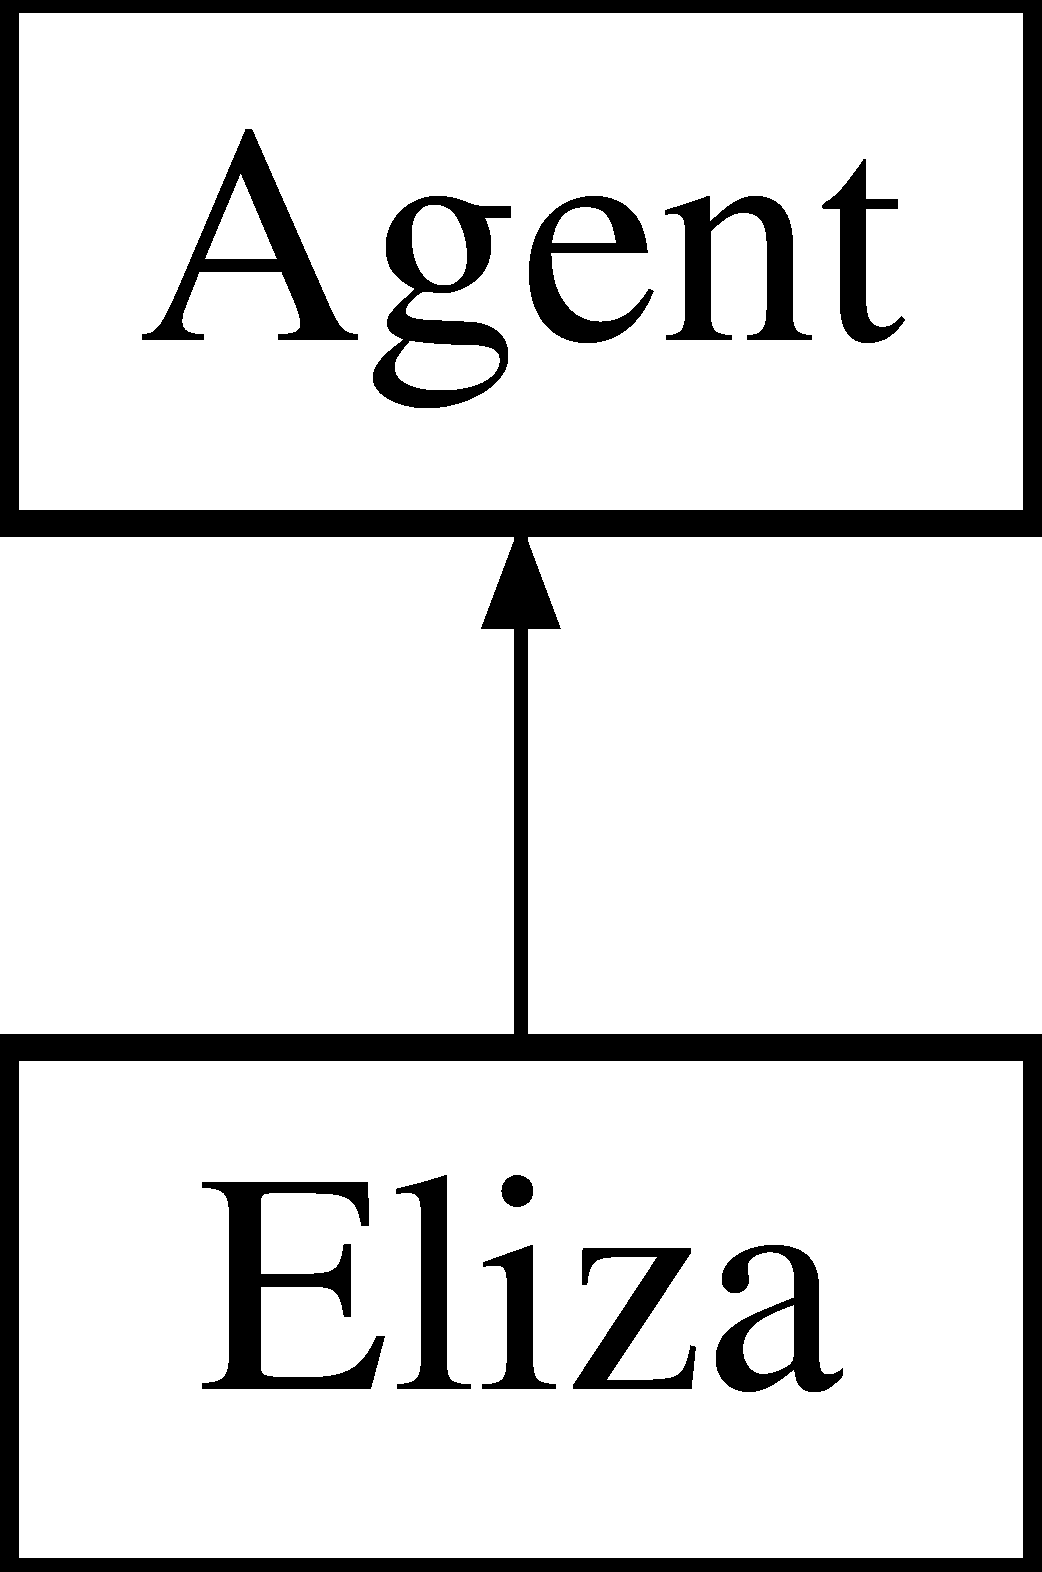
\includegraphics[height=2.000000cm]{classAgent}
\end{center}
\end{figure}
\subsection*{Public Member Functions}
\begin{DoxyCompactItemize}
\item 
\mbox{\hyperlink{classAgent_a3db4a9cfcea636c9d63ec73729225fc8}{Agent}} (istream $\ast$input, ostream $\ast$output)
\item 
void \mbox{\hyperlink{classAgent_a5e176f9a9b2a9269506cc172c1e2b897}{run}} (bool debug=false)
\end{DoxyCompactItemize}
\subsection*{Public Attributes}
\begin{DoxyCompactItemize}
\item 
\mbox{\Hypertarget{classAgent_a18b65b5aff8b98ba9316d6b75b5fc365}\label{classAgent_a18b65b5aff8b98ba9316d6b75b5fc365}} 
\mbox{\hyperlink{classString}{String}} \mbox{\hyperlink{classAgent_a18b65b5aff8b98ba9316d6b75b5fc365}{name}}
\begin{DoxyCompactList}\small\item\em \mbox{\hyperlink{classAgent}{Agent}} name. \end{DoxyCompactList}\item 
\mbox{\Hypertarget{classAgent_af9d3de27eff21068dca2e7d73f6bdd3e}\label{classAgent_af9d3de27eff21068dca2e7d73f6bdd3e}} 
istream $\ast$ \mbox{\hyperlink{classAgent_af9d3de27eff21068dca2e7d73f6bdd3e}{input\+Stream}}
\begin{DoxyCompactList}\small\item\em pointer to input stream \end{DoxyCompactList}\item 
\mbox{\Hypertarget{classAgent_ac00b0a19e22cbda3d748704b073f373a}\label{classAgent_ac00b0a19e22cbda3d748704b073f373a}} 
ostream $\ast$ \mbox{\hyperlink{classAgent_ac00b0a19e22cbda3d748704b073f373a}{output\+Stream}}
\begin{DoxyCompactList}\small\item\em pointer to output stream \end{DoxyCompactList}\item 
\mbox{\Hypertarget{classAgent_ac6d993fd4391bbd272be8bcdaeab350c}\label{classAgent_ac6d993fd4391bbd272be8bcdaeab350c}} 
bool \mbox{\hyperlink{classAgent_ac6d993fd4391bbd272be8bcdaeab350c}{quit}}
\begin{DoxyCompactList}\small\item\em boolean to quit conversation \end{DoxyCompactList}\end{DoxyCompactItemize}
\subsection*{Protected Member Functions}
\begin{DoxyCompactItemize}
\item 
virtual \mbox{\hyperlink{classString}{String}} \mbox{\hyperlink{classAgent_a8908483f8d1302ec8dd65539369de9bb}{process\+Input}} (\mbox{\hyperlink{classString}{String}} input)=0
\item 
virtual \mbox{\hyperlink{classString}{String}} \mbox{\hyperlink{classAgent_a753289e615d0fbe962453695e41bd0b6}{greet\+User}} ()=0
\end{DoxyCompactItemize}
\subsection*{Protected Attributes}
\begin{DoxyCompactItemize}
\item 
\mbox{\Hypertarget{classAgent_a5536c1d6d3beb2d9ccee127d33ceaf2e}\label{classAgent_a5536c1d6d3beb2d9ccee127d33ceaf2e}} 
ostream $\ast$ \mbox{\hyperlink{classAgent_a5536c1d6d3beb2d9ccee127d33ceaf2e}{debugger}}
\begin{DoxyCompactList}\small\item\em Pointer to output stream for displaying debug information.~\newline
Can be used to point to a file stream to write a log file. \end{DoxyCompactList}\end{DoxyCompactItemize}


\subsection{Detailed Description}
Processes input speech and generates output. 

\subsection{Constructor \& Destructor Documentation}
\mbox{\Hypertarget{classAgent_a3db4a9cfcea636c9d63ec73729225fc8}\label{classAgent_a3db4a9cfcea636c9d63ec73729225fc8}} 
\index{Agent@{Agent}!Agent@{Agent}}
\index{Agent@{Agent}!Agent@{Agent}}
\subsubsection{\texorpdfstring{Agent()}{Agent()}}
{\footnotesize\ttfamily Agent\+::\+Agent (\begin{DoxyParamCaption}\item[{istream $\ast$}]{input,  }\item[{ostream $\ast$}]{output }\end{DoxyParamCaption})}

\mbox{\hyperlink{classAgent}{Agent}} constructor that initializes I/O streams 
\begin{DoxyParams}{Parameters}
{\em input} & Pointer to input stream \\
\hline
{\em output} & Pointer to output stream \\
\hline
\end{DoxyParams}


\subsection{Member Function Documentation}
\mbox{\Hypertarget{classAgent_a753289e615d0fbe962453695e41bd0b6}\label{classAgent_a753289e615d0fbe962453695e41bd0b6}} 
\index{Agent@{Agent}!greet\+User@{greet\+User}}
\index{greet\+User@{greet\+User}!Agent@{Agent}}
\subsubsection{\texorpdfstring{greet\+User()}{greetUser()}}
{\footnotesize\ttfamily virtual \mbox{\hyperlink{classString}{String}} Agent\+::greet\+User (\begin{DoxyParamCaption}{ }\end{DoxyParamCaption})\hspace{0.3cm}{\ttfamily [protected]}, {\ttfamily [pure virtual]}}

Generates greeting at the beginning of the conversation. \begin{DoxyReturn}{Returns}
output string. 
\end{DoxyReturn}


Implemented in \mbox{\hyperlink{classEliza_a87224cd89d0e0dafbc2e8883d1a83f14}{Eliza}}.

\mbox{\Hypertarget{classAgent_a8908483f8d1302ec8dd65539369de9bb}\label{classAgent_a8908483f8d1302ec8dd65539369de9bb}} 
\index{Agent@{Agent}!process\+Input@{process\+Input}}
\index{process\+Input@{process\+Input}!Agent@{Agent}}
\subsubsection{\texorpdfstring{process\+Input()}{processInput()}}
{\footnotesize\ttfamily virtual \mbox{\hyperlink{classString}{String}} Agent\+::process\+Input (\begin{DoxyParamCaption}\item[{\mbox{\hyperlink{classString}{String}}}]{input }\end{DoxyParamCaption})\hspace{0.3cm}{\ttfamily [protected]}, {\ttfamily [pure virtual]}}

Processes input string and generates response. 
\begin{DoxyParams}{Parameters}
{\em input} & User input \\
\hline
\end{DoxyParams}
\begin{DoxyReturn}{Returns}
Processed output 
\end{DoxyReturn}


Implemented in \mbox{\hyperlink{classEliza_a9700906fb44016db11cd1183d5a1f1f3}{Eliza}}.

\mbox{\Hypertarget{classAgent_a5e176f9a9b2a9269506cc172c1e2b897}\label{classAgent_a5e176f9a9b2a9269506cc172c1e2b897}} 
\index{Agent@{Agent}!run@{run}}
\index{run@{run}!Agent@{Agent}}
\subsubsection{\texorpdfstring{run()}{run()}}
{\footnotesize\ttfamily void Agent\+::run (\begin{DoxyParamCaption}\item[{bool}]{debug = {\ttfamily false} }\end{DoxyParamCaption})}

Runs agent until \mbox{\hyperlink{classAgent_ac6d993fd4391bbd272be8bcdaeab350c}{Agent.\+quit}} is true. 
\begin{DoxyParams}{Parameters}
{\em debug} & if true, displays running processes. \\
\hline
\end{DoxyParams}


The documentation for this class was generated from the following files\+:\begin{DoxyCompactItemize}
\item 
src/\+Agent/Agent.\+h\item 
src/\+Agent/Agent.\+cpp\end{DoxyCompactItemize}

\hypertarget{classAnalyser}{}\section{Analyser Class Reference}
\label{classAnalyser}\index{Analyser@{Analyser}}


The analyser is responsible for the different parsing jobs that are used by the agent.  




{\ttfamily \#include $<$Analyser.\+h$>$}

Inheritance diagram for Analyser\+:\begin{figure}[H]
\begin{center}
\leavevmode
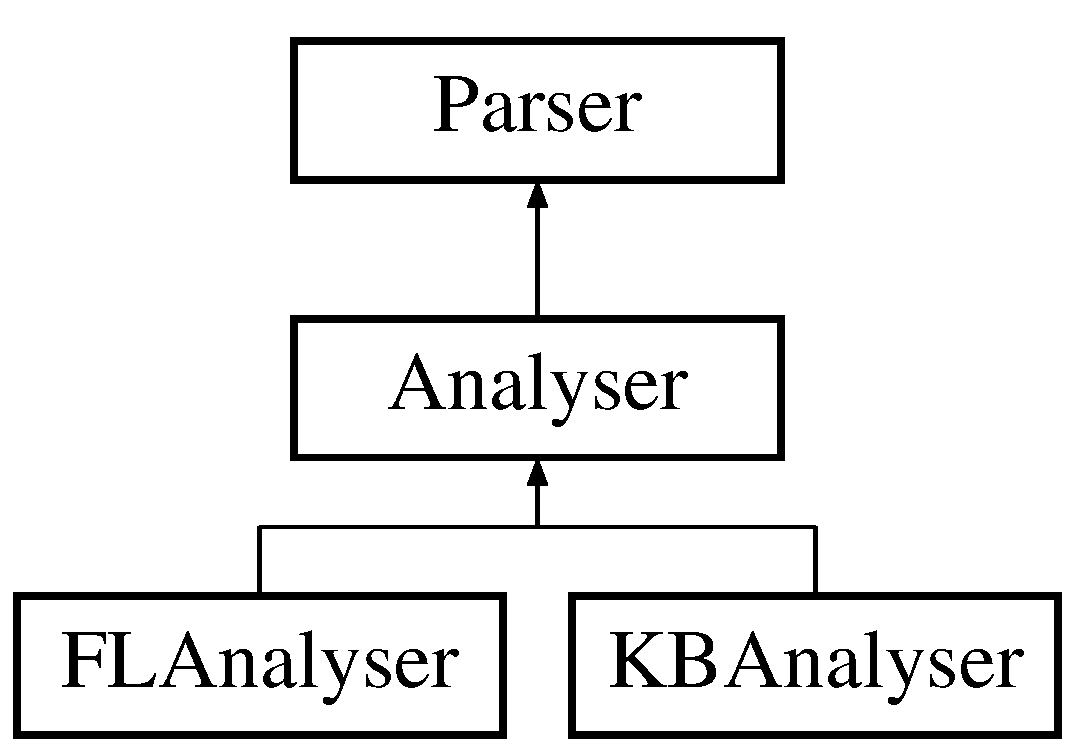
\includegraphics[height=3.000000cm]{classAnalyser}
\end{center}
\end{figure}
\subsection*{Public Member Functions}
\begin{DoxyCompactItemize}
\item 
Parse\+Tree \mbox{\hyperlink{classAnalyser_ad44df7523051fa8e152e1f623d00aa9a}{parse}} (\mbox{\hyperlink{classString}{String}} words, Grammar grammar)
\begin{DoxyCompactList}\small\item\em This function creates a parse tree given a set of words and a grammar. \end{DoxyCompactList}\end{DoxyCompactItemize}
\subsection*{Public Attributes}
\begin{DoxyCompactItemize}
\item 
Lexer \mbox{\hyperlink{classAnalyser_a4b5cb814df4274dbc426174a89b9838f}{lexer}}
\end{DoxyCompactItemize}
\subsection*{Additional Inherited Members}


\subsection{Detailed Description}
The analyser is responsible for the different parsing jobs that are used by the agent. 

\subsection{Member Function Documentation}
\mbox{\Hypertarget{classAnalyser_ad44df7523051fa8e152e1f623d00aa9a}\label{classAnalyser_ad44df7523051fa8e152e1f623d00aa9a}} 
\index{Analyser@{Analyser}!parse@{parse}}
\index{parse@{parse}!Analyser@{Analyser}}
\subsubsection{\texorpdfstring{parse()}{parse()}}
{\footnotesize\ttfamily Parse\+Tree Analyser\+::parse (\begin{DoxyParamCaption}\item[{\mbox{\hyperlink{classString}{String}}}]{words,  }\item[{Grammar}]{grammar }\end{DoxyParamCaption})}



This function creates a parse tree given a set of words and a grammar. 


\begin{DoxyParams}{Parameters}
{\em words} & The words to be transformed into a parse tree. \\
\hline
{\em grammar} & The grammar of the language in question. \\
\hline
\end{DoxyParams}
\begin{DoxyReturn}{Returns}
A parse tree. 
\end{DoxyReturn}


\subsection{Member Data Documentation}
\mbox{\Hypertarget{classAnalyser_a4b5cb814df4274dbc426174a89b9838f}\label{classAnalyser_a4b5cb814df4274dbc426174a89b9838f}} 
\index{Analyser@{Analyser}!lexer@{lexer}}
\index{lexer@{lexer}!Analyser@{Analyser}}
\subsubsection{\texorpdfstring{lexer}{lexer}}
{\footnotesize\ttfamily Lexer Analyser\+::lexer}

The lexer that is used by the analyser. 

The documentation for this class was generated from the following file\+:\begin{DoxyCompactItemize}
\item 
src/\+Agent/\+Knowledge\+Base/\mbox{\hyperlink{Analyser_8h}{Analyser.\+h}}\end{DoxyCompactItemize}

\hypertarget{classClient}{}\section{Client Class Reference}
\label{classClient}\index{Client@{Client}}


{\ttfamily \#include $<$Client.\+h$>$}

Inheritance diagram for Client\+:\begin{figure}[H]
\begin{center}
\leavevmode
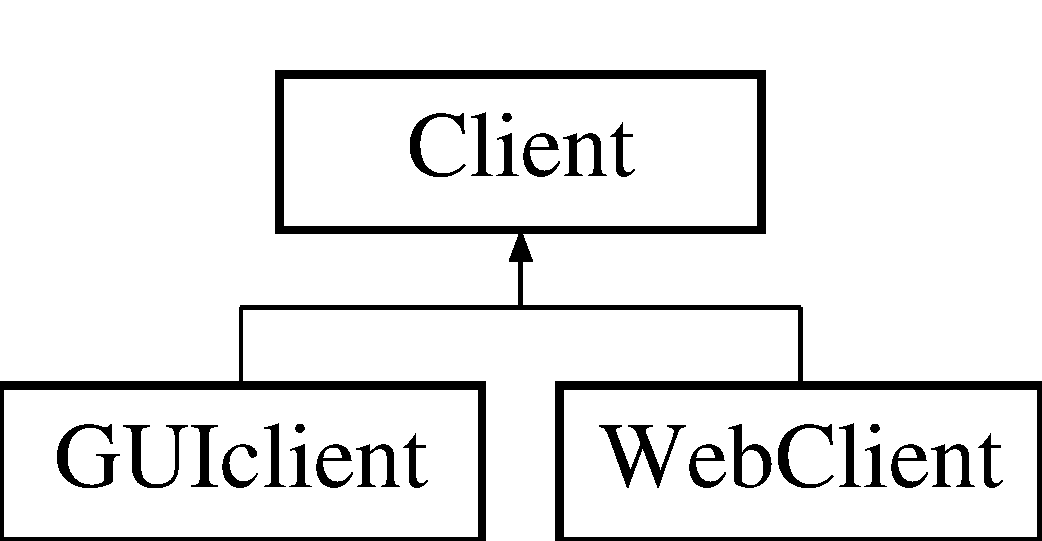
\includegraphics[height=2.000000cm]{classClient}
\end{center}
\end{figure}


\subsection{Detailed Description}
Project Chat\+Bot 

The documentation for this class was generated from the following file\+:\begin{DoxyCompactItemize}
\item 
src/\+Client/Client.\+h\end{DoxyCompactItemize}

\hypertarget{classDecomp}{}\section{Decomp Class Reference}
\label{classDecomp}\index{Decomp@{Decomp}}


Decomposition rule for a sentence.  




{\ttfamily \#include $<$Decomp.\+h$>$}

\subsection*{Public Member Functions}
\begin{DoxyCompactItemize}
\item 
\mbox{\hyperlink{classDecomp_a01a72f90b40f1f7ba98349443f3d0b1c}{Decomp}} (\mbox{\hyperlink{classKey}{Key}} $\ast$\mbox{\hyperlink{classDecomp_aac5121057365009504733971b61b5144}{key}}, \mbox{\hyperlink{classString}{String}} script\+Line, \mbox{\hyperlink{classThesaurus}{Thesaurus}} thes)
\item 
void \mbox{\hyperlink{classDecomp_a8ff1983b817d90d03b5f2726cc2e7af8}{new\+Reasmb}} (\mbox{\hyperlink{classString}{String}} reasmb)
\item 
vector$<$ \mbox{\hyperlink{classString}{String}} $>$ \mbox{\hyperlink{classDecomp_a5778e75423e33df37fe2e41157d3bc03}{decompose}} (\mbox{\hyperlink{classString}{String}} str)
\item 
\mbox{\hyperlink{classReasmb}{Reasmb}} $\ast$ \mbox{\hyperlink{classDecomp_ae3a21380fd65ef17ca0c1b4bb4aa7875}{next\+Rule}} ()
\end{DoxyCompactItemize}
\subsection*{Public Attributes}
\begin{DoxyCompactItemize}
\item 
\mbox{\Hypertarget{classDecomp_aa306bb725aade0708e3796b362b7eb50}\label{classDecomp_aa306bb725aade0708e3796b362b7eb50}} 
\mbox{\hyperlink{classString}{String}} \mbox{\hyperlink{classDecomp_aa306bb725aade0708e3796b362b7eb50}{pattern}}
\begin{DoxyCompactList}\small\item\em Decomposition R\+E\+G\+EX pattern. \end{DoxyCompactList}\item 
\mbox{\Hypertarget{classDecomp_a2ca89dea0471f80c7921955fafdf8513}\label{classDecomp_a2ca89dea0471f80c7921955fafdf8513}} 
vector$<$ \mbox{\hyperlink{classReasmb}{Reasmb}} $\ast$ $>$ \mbox{\hyperlink{classDecomp_a2ca89dea0471f80c7921955fafdf8513}{reassemb}}
\begin{DoxyCompactList}\small\item\em List of reassembly rules for decomposition. \end{DoxyCompactList}\item 
\mbox{\Hypertarget{classDecomp_aac5121057365009504733971b61b5144}\label{classDecomp_aac5121057365009504733971b61b5144}} 
\mbox{\hyperlink{classKey}{Key}} $\ast$ \mbox{\hyperlink{classDecomp_aac5121057365009504733971b61b5144}{key}}
\begin{DoxyCompactList}\small\item\em Pointer to parent \mbox{\hyperlink{classKey}{Key}}. \end{DoxyCompactList}\item 
\mbox{\Hypertarget{classDecomp_a31c944c87ebaa500f277279de14e382e}\label{classDecomp_a31c944c87ebaa500f277279de14e382e}} 
bool \mbox{\hyperlink{classDecomp_a31c944c87ebaa500f277279de14e382e}{mem}}
\begin{DoxyCompactList}\small\item\em save decomposition rule in memory ? \end{DoxyCompactList}\end{DoxyCompactItemize}
\subsection*{Private Attributes}
\begin{DoxyCompactItemize}
\item 
\mbox{\Hypertarget{classDecomp_ad0e34d40664740f5d4743474ed607262}\label{classDecomp_ad0e34d40664740f5d4743474ed607262}} 
size\+\_\+t \mbox{\hyperlink{classDecomp_ad0e34d40664740f5d4743474ed607262}{reassemb\+Rule}} = -\/1
\begin{DoxyCompactList}\small\item\em current reassembly rule index in \mbox{\hyperlink{classDecomp_a2ca89dea0471f80c7921955fafdf8513}{Decomp.\+reassemb}}, -\/1 if not assigned. \end{DoxyCompactList}\end{DoxyCompactItemize}
\subsection*{Friends}
\begin{DoxyCompactItemize}
\item 
\mbox{\Hypertarget{classDecomp_aca677c336732ff9d6ac1d4ac6f000dd7}\label{classDecomp_aca677c336732ff9d6ac1d4ac6f000dd7}} 
ostream \& {\bfseries operator$<$$<$} (ostream \&os, const \mbox{\hyperlink{classDecomp}{Decomp}} \&decomp)
\end{DoxyCompactItemize}


\subsection{Detailed Description}
Decomposition rule for a sentence. 

\subsection{Constructor \& Destructor Documentation}
\mbox{\Hypertarget{classDecomp_a01a72f90b40f1f7ba98349443f3d0b1c}\label{classDecomp_a01a72f90b40f1f7ba98349443f3d0b1c}} 
\index{Decomp@{Decomp}!Decomp@{Decomp}}
\index{Decomp@{Decomp}!Decomp@{Decomp}}
\subsubsection{\texorpdfstring{Decomp()}{Decomp()}}
{\footnotesize\ttfamily Decomp\+::\+Decomp (\begin{DoxyParamCaption}\item[{\mbox{\hyperlink{classKey}{Key}} $\ast$}]{key,  }\item[{\mbox{\hyperlink{classString}{String}}}]{script\+Line,  }\item[{\mbox{\hyperlink{classThesaurus}{Thesaurus}}}]{thes }\end{DoxyParamCaption})}

Default constructor, translates script pattern (special format) into R\+E\+G\+EX. 
\begin{DoxyParams}{Parameters}
{\em key} & parent \mbox{\hyperlink{classKey}{Key}} \\
\hline
{\em script\+Line} & output string from \mbox{\hyperlink{classScript_a946d037839b4caada09e22a428c8f42e}{Script\+::extract\+Pattern}} \\
\hline
{\em thes} & \mbox{\hyperlink{classThesaurus}{Thesaurus}} object \\
\hline
\end{DoxyParams}


\subsection{Member Function Documentation}
\mbox{\Hypertarget{classDecomp_a5778e75423e33df37fe2e41157d3bc03}\label{classDecomp_a5778e75423e33df37fe2e41157d3bc03}} 
\index{Decomp@{Decomp}!decompose@{decompose}}
\index{decompose@{decompose}!Decomp@{Decomp}}
\subsubsection{\texorpdfstring{decompose()}{decompose()}}
{\footnotesize\ttfamily vector$<$ \mbox{\hyperlink{classString}{String}} $>$ Decomp\+::decompose (\begin{DoxyParamCaption}\item[{\mbox{\hyperlink{classString}{String}}}]{str }\end{DoxyParamCaption})}

Decomposes a sentence according. 
\begin{DoxyParams}{Parameters}
{\em str} & input sentence \\
\hline
\end{DoxyParams}
\begin{DoxyReturn}{Returns}
vector of matching expressions 
\end{DoxyReturn}
\mbox{\Hypertarget{classDecomp_a8ff1983b817d90d03b5f2726cc2e7af8}\label{classDecomp_a8ff1983b817d90d03b5f2726cc2e7af8}} 
\index{Decomp@{Decomp}!new\+Reasmb@{new\+Reasmb}}
\index{new\+Reasmb@{new\+Reasmb}!Decomp@{Decomp}}
\subsubsection{\texorpdfstring{new\+Reasmb()}{newReasmb()}}
{\footnotesize\ttfamily void Decomp\+::new\+Reasmb (\begin{DoxyParamCaption}\item[{\mbox{\hyperlink{classString}{String}}}]{reasmb }\end{DoxyParamCaption})}

Creates new reassembly object, adds it to \mbox{\hyperlink{classDecomp_a2ca89dea0471f80c7921955fafdf8513}{Decomp.\+reassemb}} and links it with the parent \mbox{\hyperlink{classDecomp}{Decomp}} object. 
\begin{DoxyParams}{Parameters}
{\em reasmb} & reassembly rule pattern. \\
\hline
\end{DoxyParams}
\mbox{\Hypertarget{classDecomp_ae3a21380fd65ef17ca0c1b4bb4aa7875}\label{classDecomp_ae3a21380fd65ef17ca0c1b4bb4aa7875}} 
\index{Decomp@{Decomp}!next\+Rule@{next\+Rule}}
\index{next\+Rule@{next\+Rule}!Decomp@{Decomp}}
\subsubsection{\texorpdfstring{next\+Rule()}{nextRule()}}
{\footnotesize\ttfamily \mbox{\hyperlink{classReasmb}{Reasmb}} $\ast$ Decomp\+::next\+Rule (\begin{DoxyParamCaption}{ }\end{DoxyParamCaption})}

\begin{DoxyReturn}{Returns}
pointer to a random rassembly rule 
\end{DoxyReturn}


The documentation for this class was generated from the following files\+:\begin{DoxyCompactItemize}
\item 
src/\+Agent/\+E\+L\+I\+Z\+A/Decomp.\+h\item 
src/\+Agent/\+E\+L\+I\+Z\+A/Decomp.\+cpp\end{DoxyCompactItemize}

\hypertarget{classEliza}{}\section{Eliza Class Reference}
\label{classEliza}\index{Eliza@{Eliza}}


\mbox{\hyperlink{classAgent}{Agent}} based on Weizenbaum\textquotesingle{}s E\+L\+I\+ZA conversational agent.  




{\ttfamily \#include $<$Eliza.\+h$>$}

Inheritance diagram for Eliza\+:\begin{figure}[H]
\begin{center}
\leavevmode
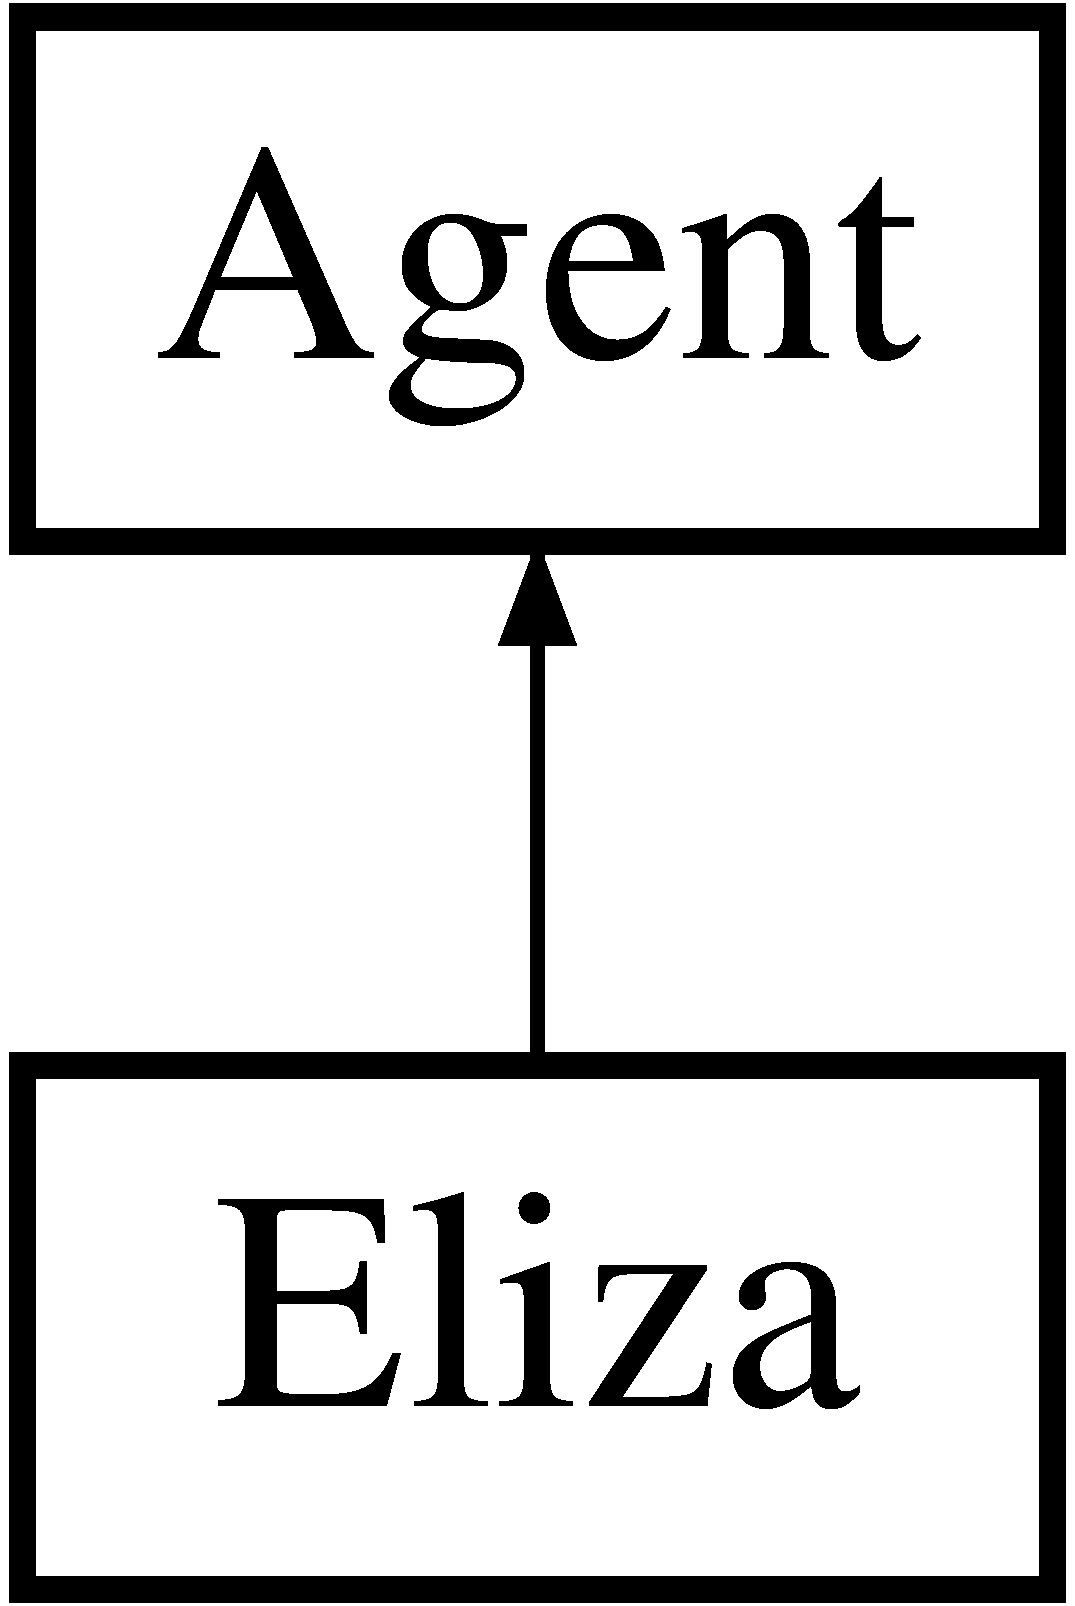
\includegraphics[height=2.000000cm]{classEliza}
\end{center}
\end{figure}
\subsection*{Public Member Functions}
\begin{DoxyCompactItemize}
\item 
\mbox{\hyperlink{classEliza_a6246b8f323f27e7b5762560ad4ad7c11}{Eliza}} (istream $\ast$input, ostream $\ast$output, \mbox{\hyperlink{classString}{String}} source\+Path)
\end{DoxyCompactItemize}
\subsection*{Public Attributes}
\begin{DoxyCompactItemize}
\item 
\mbox{\Hypertarget{classEliza_aa4f2c7a48333da7b14c5e24c1bd49f51}\label{classEliza_aa4f2c7a48333da7b14c5e24c1bd49f51}} 
\mbox{\hyperlink{classScript}{Script}} $\ast$ \mbox{\hyperlink{classEliza_aa4f2c7a48333da7b14c5e24c1bd49f51}{script}}
\begin{DoxyCompactList}\small\item\em Database parser for E\+L\+I\+ZA. \end{DoxyCompactList}\item 
\mbox{\Hypertarget{classEliza_a2414a3a9a6e096752a27ae5140068c17}\label{classEliza_a2414a3a9a6e096752a27ae5140068c17}} 
\mbox{\hyperlink{classMemory}{Memory}} \mbox{\hyperlink{classEliza_a2414a3a9a6e096752a27ae5140068c17}{memory}}
\begin{DoxyCompactList}\small\item\em \mbox{\hyperlink{classMemory}{Memory}} stack. \end{DoxyCompactList}\end{DoxyCompactItemize}
\subsection*{Private Member Functions}
\begin{DoxyCompactItemize}
\item 
\mbox{\hyperlink{classString}{String}} \mbox{\hyperlink{classEliza_a9700906fb44016db11cd1183d5a1f1f3}{process\+Input}} (\mbox{\hyperlink{classString}{String}} input) override
\item 
\mbox{\hyperlink{classString}{String}} \mbox{\hyperlink{classEliza_a87224cd89d0e0dafbc2e8883d1a83f14}{greet\+User}} () override
\item 
vector$<$ \mbox{\hyperlink{classKey}{Key}} $\ast$ $>$ \mbox{\hyperlink{classEliza_adb573920365f86efd4974fa1af6e4f47}{collect\+Keys}} (\mbox{\hyperlink{classString}{String}} input)
\item 
\mbox{\hyperlink{classString}{String}} \mbox{\hyperlink{classEliza_a388dad084acdf7310dc1028bdee044f2}{process\+Sentence}} (\mbox{\hyperlink{classString}{String}} input)
\item 
\mbox{\hyperlink{classString}{String}} \mbox{\hyperlink{classEliza_a74fbfaf3553aa9224ba10ef0881d6f14}{decompose\+On\+Key}} (\mbox{\hyperlink{classDecomp}{Decomp}} $\ast$decomp, \mbox{\hyperlink{classString}{String}} input)
\end{DoxyCompactItemize}
\subsection*{Additional Inherited Members}


\subsection{Detailed Description}
\mbox{\hyperlink{classAgent}{Agent}} based on Weizenbaum\textquotesingle{}s E\+L\+I\+ZA conversational agent. 

\subsection{Constructor \& Destructor Documentation}
\mbox{\Hypertarget{classEliza_a6246b8f323f27e7b5762560ad4ad7c11}\label{classEliza_a6246b8f323f27e7b5762560ad4ad7c11}} 
\index{Eliza@{Eliza}!Eliza@{Eliza}}
\index{Eliza@{Eliza}!Eliza@{Eliza}}
\subsubsection{\texorpdfstring{Eliza()}{Eliza()}}
{\footnotesize\ttfamily Eliza\+::\+Eliza (\begin{DoxyParamCaption}\item[{istream $\ast$}]{input,  }\item[{ostream $\ast$}]{output,  }\item[{\mbox{\hyperlink{classString}{String}}}]{source\+Path }\end{DoxyParamCaption})}

Default constructor for \mbox{\hyperlink{classEliza}{Eliza}}. Calls inherited constructor and sets \mbox{\hyperlink{classAgent_a18b65b5aff8b98ba9316d6b75b5fc365}{Agent.\+name}} and memory. See \mbox{\hyperlink{classAgent_a3db4a9cfcea636c9d63ec73729225fc8}{Agent.\+Agent()}} 

\subsection{Member Function Documentation}
\mbox{\Hypertarget{classEliza_adb573920365f86efd4974fa1af6e4f47}\label{classEliza_adb573920365f86efd4974fa1af6e4f47}} 
\index{Eliza@{Eliza}!collect\+Keys@{collect\+Keys}}
\index{collect\+Keys@{collect\+Keys}!Eliza@{Eliza}}
\subsubsection{\texorpdfstring{collect\+Keys()}{collectKeys()}}
{\footnotesize\ttfamily vector$<$ \mbox{\hyperlink{classKey}{Key}} $\ast$ $>$ Eliza\+::collect\+Keys (\begin{DoxyParamCaption}\item[{\mbox{\hyperlink{classString}{String}}}]{input }\end{DoxyParamCaption})\hspace{0.3cm}{\ttfamily [private]}}

Collects keywords from user input. 
\begin{DoxyParams}{Parameters}
{\em input} & user input \\
\hline
\end{DoxyParams}
\begin{DoxyReturn}{Returns}
keywords (sorted in descending order according to \mbox{\hyperlink{classKey_ad960b9e4804c3cb039a816811bae4839}{Key\+::rank}}) 
\end{DoxyReturn}
\mbox{\Hypertarget{classEliza_a74fbfaf3553aa9224ba10ef0881d6f14}\label{classEliza_a74fbfaf3553aa9224ba10ef0881d6f14}} 
\index{Eliza@{Eliza}!decompose\+On\+Key@{decompose\+On\+Key}}
\index{decompose\+On\+Key@{decompose\+On\+Key}!Eliza@{Eliza}}
\subsubsection{\texorpdfstring{decompose\+On\+Key()}{decomposeOnKey()}}
{\footnotesize\ttfamily \mbox{\hyperlink{classString}{String}} Eliza\+::decompose\+On\+Key (\begin{DoxyParamCaption}\item[{\mbox{\hyperlink{classDecomp}{Decomp}} $\ast$}]{decomp,  }\item[{\mbox{\hyperlink{classString}{String}}}]{input }\end{DoxyParamCaption})\hspace{0.3cm}{\ttfamily [private]}}

Decomposes input string on given decomposition rule. Calls\+:
\begin{DoxyItemize}
\item vector$<$\+String$>$ decomp\+::decompose(\+String input)
\item Reasmb$\ast$ decomp\+::next\+Rule()
\item \mbox{\hyperlink{classString}{String}} reasmb\+::reassemble(vector$<$\+String$>$ matches) 
\begin{DoxyParams}{Parameters}
{\em decomp} & pointer to decomposition rule \\
\hline
{\em input} & input string \\
\hline
\end{DoxyParams}
\begin{DoxyReturn}{Returns}
reassembled string 
\end{DoxyReturn}

\end{DoxyItemize}\mbox{\Hypertarget{classEliza_a87224cd89d0e0dafbc2e8883d1a83f14}\label{classEliza_a87224cd89d0e0dafbc2e8883d1a83f14}} 
\index{Eliza@{Eliza}!greet\+User@{greet\+User}}
\index{greet\+User@{greet\+User}!Eliza@{Eliza}}
\subsubsection{\texorpdfstring{greet\+User()}{greetUser()}}
{\footnotesize\ttfamily \mbox{\hyperlink{classString}{String}} Eliza\+::greet\+User (\begin{DoxyParamCaption}{ }\end{DoxyParamCaption})\hspace{0.3cm}{\ttfamily [override]}, {\ttfamily [private]}, {\ttfamily [virtual]}}

Generates greeting at the beginning of the conversation. \begin{DoxyReturn}{Returns}
output string. 
\end{DoxyReturn}


Implements \mbox{\hyperlink{classAgent_a753289e615d0fbe962453695e41bd0b6}{Agent}}.

\mbox{\Hypertarget{classEliza_a9700906fb44016db11cd1183d5a1f1f3}\label{classEliza_a9700906fb44016db11cd1183d5a1f1f3}} 
\index{Eliza@{Eliza}!process\+Input@{process\+Input}}
\index{process\+Input@{process\+Input}!Eliza@{Eliza}}
\subsubsection{\texorpdfstring{process\+Input()}{processInput()}}
{\footnotesize\ttfamily \mbox{\hyperlink{classString}{String}} Eliza\+::process\+Input (\begin{DoxyParamCaption}\item[{\mbox{\hyperlink{classString}{String}}}]{input }\end{DoxyParamCaption})\hspace{0.3cm}{\ttfamily [override]}, {\ttfamily [private]}, {\ttfamily [virtual]}}

Processes input string and generates response. 
\begin{DoxyParams}{Parameters}
{\em input} & User input \\
\hline
\end{DoxyParams}
\begin{DoxyReturn}{Returns}
Processed output 
\end{DoxyReturn}


Implements \mbox{\hyperlink{classAgent_a8908483f8d1302ec8dd65539369de9bb}{Agent}}.

\mbox{\Hypertarget{classEliza_a388dad084acdf7310dc1028bdee044f2}\label{classEliza_a388dad084acdf7310dc1028bdee044f2}} 
\index{Eliza@{Eliza}!process\+Sentence@{process\+Sentence}}
\index{process\+Sentence@{process\+Sentence}!Eliza@{Eliza}}
\subsubsection{\texorpdfstring{process\+Sentence()}{processSentence()}}
{\footnotesize\ttfamily \mbox{\hyperlink{classString}{String}} Eliza\+::process\+Sentence (\begin{DoxyParamCaption}\item[{\mbox{\hyperlink{classString}{String}}}]{input }\end{DoxyParamCaption})\hspace{0.3cm}{\ttfamily [private]}}

Process individual sentences from input. 
\begin{DoxyParams}{Parameters}
{\em input} & broken user sentence \\
\hline
\end{DoxyParams}
\begin{DoxyReturn}{Returns}
processed answer 
\end{DoxyReturn}


The documentation for this class was generated from the following files\+:\begin{DoxyCompactItemize}
\item 
src/\+Agent/\+E\+L\+I\+Z\+A/Eliza.\+h\item 
src/\+Agent/\+E\+L\+I\+Z\+A/Eliza.\+cpp\end{DoxyCompactItemize}

\hypertarget{classFLAnalyser}{}\section{F\+L\+Analyser Class Reference}
\label{classFLAnalyser}\index{F\+L\+Analyser@{F\+L\+Analyser}}


This class uses the parse tree generated by the parser and translates it into a formal language (a small set of the English language in this case)  




{\ttfamily \#include $<$F\+L\+Analyser.\+h$>$}

Inheritance diagram for F\+L\+Analyser\+:\begin{figure}[H]
\begin{center}
\leavevmode
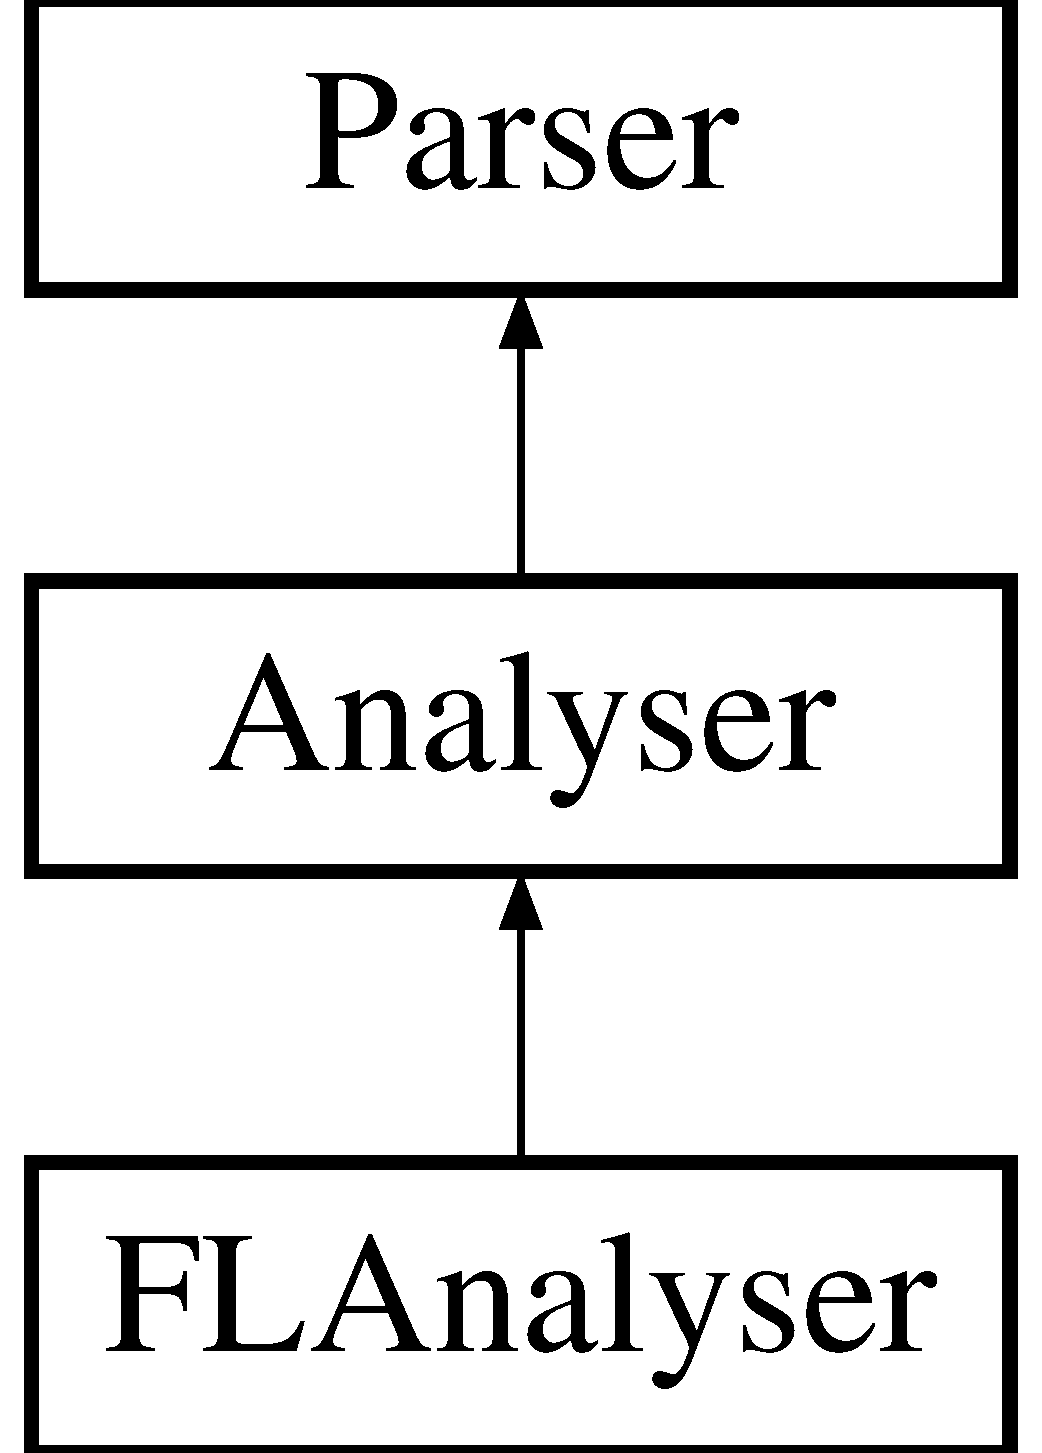
\includegraphics[height=3.000000cm]{classFLAnalyser}
\end{center}
\end{figure}
\subsection*{Public Member Functions}
\begin{DoxyCompactItemize}
\item 
vector$<$ \mbox{\hyperlink{classSentence}{Sentence}} $>$ \mbox{\hyperlink{classFLAnalyser_a5ed65a6b9033106c9b6ca5c6a7b8e45f}{interpret}} ()
\begin{DoxyCompactList}\small\item\em This function interprets the parse tree and gives equivalent possible intepretations of the tree. \end{DoxyCompactList}\item 
vector$<$ \mbox{\hyperlink{classSentence}{Sentence}} $>$ \mbox{\hyperlink{classFLAnalyser_ac842959db593592a80f3e2e8508c22c1}{disambiguate}} (vector$<$ vector$<$ \mbox{\hyperlink{classSentence}{Sentence}} $>$$>$ ps)
\begin{DoxyCompactList}\small\item\em This function disambiguates the different interpreted sentences in order to pick the one that makes the most sense. \end{DoxyCompactList}\end{DoxyCompactItemize}
\subsection*{Public Attributes}
\begin{DoxyCompactItemize}
\item 
Parse\+Tree \mbox{\hyperlink{classFLAnalyser_ad5708840f0ea357a2f81c240b16da54a}{t}}
\end{DoxyCompactItemize}
\subsection*{Additional Inherited Members}


\subsection{Detailed Description}
This class uses the parse tree generated by the parser and translates it into a formal language (a small set of the English language in this case) 

\subsection{Member Function Documentation}
\mbox{\Hypertarget{classFLAnalyser_ac842959db593592a80f3e2e8508c22c1}\label{classFLAnalyser_ac842959db593592a80f3e2e8508c22c1}} 
\index{F\+L\+Analyser@{F\+L\+Analyser}!disambiguate@{disambiguate}}
\index{disambiguate@{disambiguate}!F\+L\+Analyser@{F\+L\+Analyser}}
\subsubsection{\texorpdfstring{disambiguate()}{disambiguate()}}
{\footnotesize\ttfamily vector$<$ \mbox{\hyperlink{classSentence}{Sentence}} $>$ F\+L\+Analyser\+::disambiguate (\begin{DoxyParamCaption}\item[{vector$<$ vector$<$ \mbox{\hyperlink{classSentence}{Sentence}} $>$$>$}]{ps }\end{DoxyParamCaption})}



This function disambiguates the different interpreted sentences in order to pick the one that makes the most sense. 


\begin{DoxyParams}{Parameters}
{\em ps} & A set of possible sentences. \\
\hline
\end{DoxyParams}
\begin{DoxyReturn}{Returns}
The correct intepretation of a sentence. 
\end{DoxyReturn}
\mbox{\Hypertarget{classFLAnalyser_a5ed65a6b9033106c9b6ca5c6a7b8e45f}\label{classFLAnalyser_a5ed65a6b9033106c9b6ca5c6a7b8e45f}} 
\index{F\+L\+Analyser@{F\+L\+Analyser}!interpret@{interpret}}
\index{interpret@{interpret}!F\+L\+Analyser@{F\+L\+Analyser}}
\subsubsection{\texorpdfstring{interpret()}{interpret()}}
{\footnotesize\ttfamily vector$<$ \mbox{\hyperlink{classSentence}{Sentence}} $>$ F\+L\+Analyser\+::interpret (\begin{DoxyParamCaption}{ }\end{DoxyParamCaption})}



This function interprets the parse tree and gives equivalent possible intepretations of the tree. 

\begin{DoxyReturn}{Returns}
Intepreted sentence. 
\end{DoxyReturn}


\subsection{Member Data Documentation}
\mbox{\Hypertarget{classFLAnalyser_ad5708840f0ea357a2f81c240b16da54a}\label{classFLAnalyser_ad5708840f0ea357a2f81c240b16da54a}} 
\index{F\+L\+Analyser@{F\+L\+Analyser}!t@{t}}
\index{t@{t}!F\+L\+Analyser@{F\+L\+Analyser}}
\subsubsection{\texorpdfstring{t}{t}}
{\footnotesize\ttfamily Parse\+Tree F\+L\+Analyser\+::t}

Parse tree used by the formal language analyser. 

The documentation for this class was generated from the following files\+:\begin{DoxyCompactItemize}
\item 
src/\+Agent/\+Knowledge\+Base/\mbox{\hyperlink{FLAnalyser_8h}{F\+L\+Analyser.\+h}}\item 
src/\+Agent/\+Knowledge\+Base/F\+L\+Analyser.\+cpp\end{DoxyCompactItemize}

\hypertarget{classGUIclient}{}\section{G\+U\+Iclient Class Reference}
\label{classGUIclient}\index{G\+U\+Iclient@{G\+U\+Iclient}}


{\ttfamily \#include $<$G\+U\+Iclient.\+h$>$}

Inheritance diagram for G\+U\+Iclient\+:\begin{figure}[H]
\begin{center}
\leavevmode
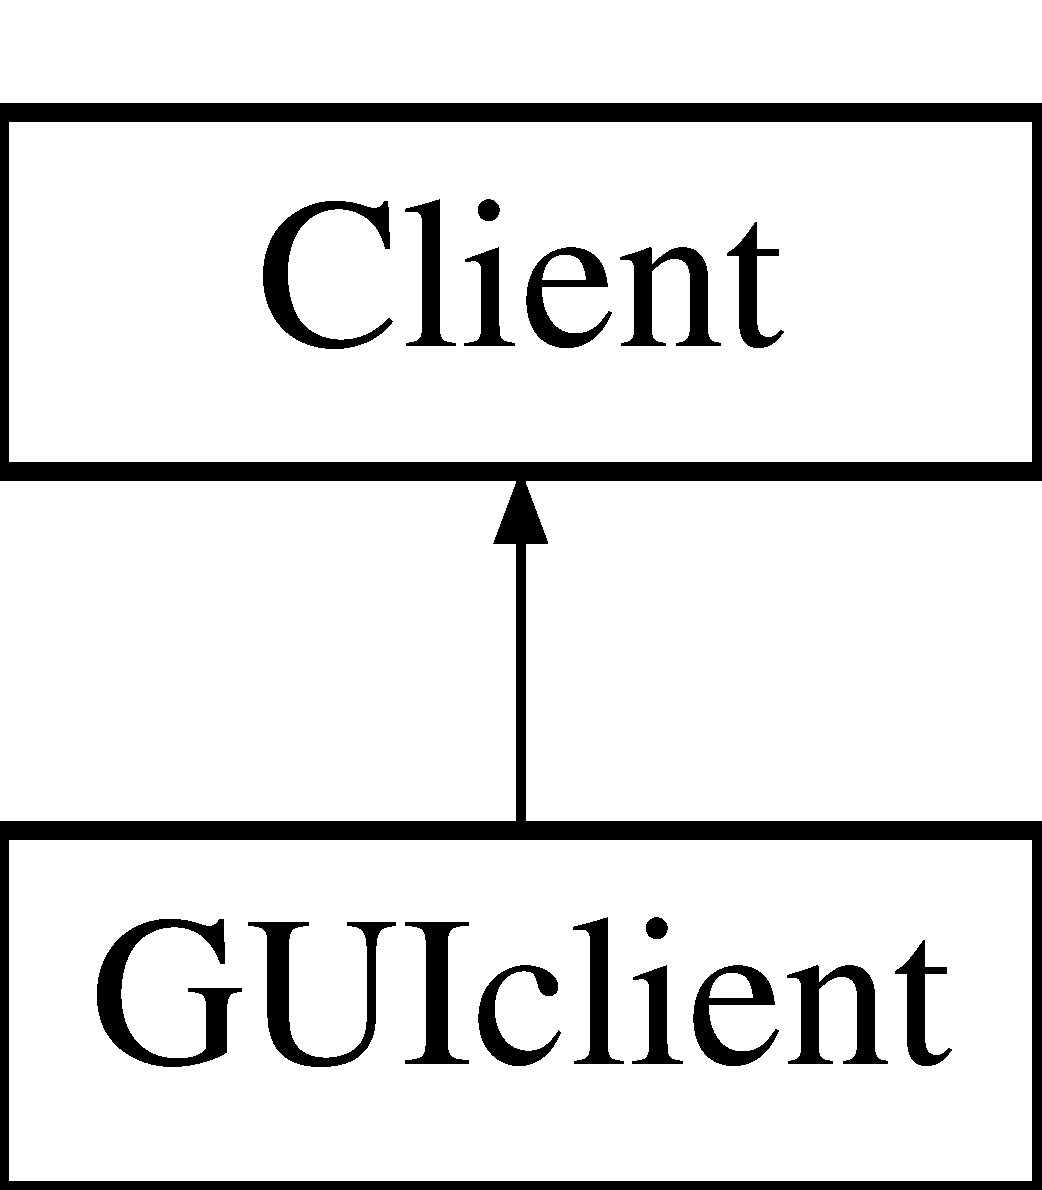
\includegraphics[height=2.000000cm]{classGUIclient}
\end{center}
\end{figure}
\subsection*{Public Member Functions}
\begin{DoxyCompactItemize}
\item 
void \mbox{\hyperlink{classGUIclient_aa78d5fe6aabaa8777bf79c60ba6ec301}{Main}} (int exit\+\_\+status)
\end{DoxyCompactItemize}


\subsection{Detailed Description}
Project Chat\+Bot 

\subsection{Member Function Documentation}
\mbox{\Hypertarget{classGUIclient_aa78d5fe6aabaa8777bf79c60ba6ec301}\label{classGUIclient_aa78d5fe6aabaa8777bf79c60ba6ec301}} 
\index{G\+U\+Iclient@{G\+U\+Iclient}!Main@{Main}}
\index{Main@{Main}!G\+U\+Iclient@{G\+U\+Iclient}}
\subsubsection{\texorpdfstring{Main()}{Main()}}
{\footnotesize\ttfamily void G\+U\+Iclient\+::\+Main (\begin{DoxyParamCaption}\item[{int}]{exit\+\_\+status }\end{DoxyParamCaption})}


\begin{DoxyParams}{Parameters}
{\em exit\+\_\+status} & Project Chat\+Bot \mbox{\hyperlink{classGUIclient}{G\+U\+Iclient}} implementation \\
\hline
{\em exit\+\_\+status} & \\
\hline
\end{DoxyParams}


The documentation for this class was generated from the following files\+:\begin{DoxyCompactItemize}
\item 
src/\+Client/\+G\+U\+I/G\+U\+Iclient.\+h\item 
src/\+Client/\+G\+U\+I/G\+U\+Iclient.\+cpp\end{DoxyCompactItemize}

\hypertarget{classKB}{}\section{KB Class Reference}
\label{classKB}\index{KB@{KB}}


This class represents our knowledge base.  




{\ttfamily \#include $<$K\+B.\+h$>$}

\subsection*{Public Member Functions}
\begin{DoxyCompactItemize}
\item 
void \mbox{\hyperlink{classKB_ab0b72bc95f5f3cd72ec0d01a10310b9f}{tell}} (\mbox{\hyperlink{classKB}{KB}} kb, vector$<$ \mbox{\hyperlink{classSentence}{Sentence}} $>$ s)
\begin{DoxyCompactList}\small\item\em This function adds a new rule to the knowledge base. \end{DoxyCompactList}\item 
vector$<$ \mbox{\hyperlink{classSentence}{Sentence}} $>$ \mbox{\hyperlink{classKB_a12ab1eba4e3792f802c943163a308518}{ask}} (\mbox{\hyperlink{classKB}{KB}} kb, vector$<$ \mbox{\hyperlink{classSentence}{Sentence}} $>$ s)
\begin{DoxyCompactList}\small\item\em This function queries the knowledge base and presents the best course of action for the agent to undertake. \end{DoxyCompactList}\item 
bool \mbox{\hyperlink{classKB_afd8d8289f3a2e60e2118b822f5c99576}{entails}} (\mbox{\hyperlink{classKB}{KB}} kb, vector$<$ \mbox{\hyperlink{classSentence}{Sentence}} $>$ s)
\begin{DoxyCompactList}\small\item\em This function checks if a new rule/sentence is logical accordance with the existant rules. \end{DoxyCompactList}\item 
void \mbox{\hyperlink{classKB_a1d77685c04f42bb2fba29ed81773dbc7}{forward\+Chain}} (\mbox{\hyperlink{classKB}{KB}} kb, vector$<$ \mbox{\hyperlink{classSentence}{Sentence}} $>$ s)
\begin{DoxyCompactList}\small\item\em This function is responsible for deducing new sentences/rules from already existing ones by using the forward chain algorithm. \end{DoxyCompactList}\item 
bool \mbox{\hyperlink{classKB_a27a8db9fc36354f1f6eb247dfcb58adc}{backward\+Chain}} (\mbox{\hyperlink{classKB}{KB}} kb, vector$<$ \mbox{\hyperlink{classSentence}{Sentence}} $>$ query)
\begin{DoxyCompactList}\small\item\em This function is used in itself by the query mechanism in order to infer whether a certain course of action is valid of production following the rules. \end{DoxyCompactList}\item 
vector$<$ \mbox{\hyperlink{classSentence}{Sentence}} $>$ \mbox{\hyperlink{classKB_abbd192b58b489d5123d844b11e1b6355}{train}} (vector$<$ vector$<$ \mbox{\hyperlink{classSentence}{Sentence}} $>$$>$ examples)
\begin{DoxyCompactList}\small\item\em This function is used to train the agent (by altering the knowledge base) based on different given hypothesis. \end{DoxyCompactList}\item 
int \mbox{\hyperlink{classKB_acc8495060f0899308126bb8487d970a6}{nb\+Rules}} (\mbox{\hyperlink{classKB}{KB}} kb)
\begin{DoxyCompactList}\small\item\em Calculates the number of rules in a knowledge base. \end{DoxyCompactList}\item 
int \mbox{\hyperlink{classKB_abbca13393d5297fcff834849272b98a9}{nb\+Facts}} (\mbox{\hyperlink{classKB}{KB}} kn)
\begin{DoxyCompactList}\small\item\em Calculates the number of facts present in a knowledge base. \end{DoxyCompactList}\end{DoxyCompactItemize}
\subsection*{Private Attributes}
\begin{DoxyCompactItemize}
\item 
vector$<$ \mbox{\hyperlink{classSentence}{Sentence}} $>$ \mbox{\hyperlink{classKB_abf6528e5e8b106c9ec57dc6a8fb86ee7}{facts}}
\item 
\mbox{\hyperlink{classKBAnalyser}{K\+B\+Analyser}} \mbox{\hyperlink{classKB_ac8dc8b51b72a89ba4c88bbc93c40b948}{analyser}}
\item 
C\+NF \mbox{\hyperlink{classKB_a810edf2192bea36c1ec95f4610fc669b}{cnfclause}}
\item 
vector$<$ Rule $>$ \mbox{\hyperlink{classKB_a41204b166f5cf54eac4d59df9f43c07a}{rules}}
\end{DoxyCompactItemize}


\subsection{Detailed Description}
This class represents our knowledge base. 

The knowledge base holds all the logical sentences and facts which can later be used to infer new facts, ask the database and train the aforementioned. 

\subsection{Member Function Documentation}
\mbox{\Hypertarget{classKB_a12ab1eba4e3792f802c943163a308518}\label{classKB_a12ab1eba4e3792f802c943163a308518}} 
\index{KB@{KB}!ask@{ask}}
\index{ask@{ask}!KB@{KB}}
\subsubsection{\texorpdfstring{ask()}{ask()}}
{\footnotesize\ttfamily vector$<$ \mbox{\hyperlink{classSentence}{Sentence}} $>$ K\+B\+::ask (\begin{DoxyParamCaption}\item[{\mbox{\hyperlink{classKB}{KB}}}]{kb,  }\item[{vector$<$ \mbox{\hyperlink{classSentence}{Sentence}} $>$}]{s }\end{DoxyParamCaption})}



This function queries the knowledge base and presents the best course of action for the agent to undertake. 


\begin{DoxyParams}{Parameters}
{\em kb} & The knowledge base. \\
\hline
{\em s} & A question in the form of a logical sentence. \\
\hline
\end{DoxyParams}
\begin{DoxyReturn}{Returns}
An action in the form of a sentence. 
\end{DoxyReturn}
\mbox{\Hypertarget{classKB_a27a8db9fc36354f1f6eb247dfcb58adc}\label{classKB_a27a8db9fc36354f1f6eb247dfcb58adc}} 
\index{KB@{KB}!backward\+Chain@{backward\+Chain}}
\index{backward\+Chain@{backward\+Chain}!KB@{KB}}
\subsubsection{\texorpdfstring{backward\+Chain()}{backwardChain()}}
{\footnotesize\ttfamily bool K\+B\+::backward\+Chain (\begin{DoxyParamCaption}\item[{\mbox{\hyperlink{classKB}{KB}}}]{kb,  }\item[{vector$<$ \mbox{\hyperlink{classSentence}{Sentence}} $>$}]{query }\end{DoxyParamCaption})}



This function is used in itself by the query mechanism in order to infer whether a certain course of action is valid of production following the rules. 


\begin{DoxyParams}{Parameters}
{\em kb} & The knowledge base \\
\hline
{\em query} & A question in the form of a logical sentence \\
\hline
\end{DoxyParams}
\begin{DoxyReturn}{Returns}
true If the proposed query is valid. 

false If the proposed query bears logical invalidity. 
\end{DoxyReturn}
\mbox{\Hypertarget{classKB_afd8d8289f3a2e60e2118b822f5c99576}\label{classKB_afd8d8289f3a2e60e2118b822f5c99576}} 
\index{KB@{KB}!entails@{entails}}
\index{entails@{entails}!KB@{KB}}
\subsubsection{\texorpdfstring{entails()}{entails()}}
{\footnotesize\ttfamily bool K\+B\+::entails (\begin{DoxyParamCaption}\item[{\mbox{\hyperlink{classKB}{KB}}}]{kb,  }\item[{vector$<$ \mbox{\hyperlink{classSentence}{Sentence}} $>$}]{s }\end{DoxyParamCaption})}



This function checks if a new rule/sentence is logical accordance with the existant rules. 


\begin{DoxyParams}{Parameters}
{\em kb} & The knowledge base. \\
\hline
{\em s} & A logical sentence. \\
\hline
\end{DoxyParams}
\begin{DoxyReturn}{Returns}
true If the sentence is in accordance with the existant rules. 

false If the sentence clashes with the existant rules. 
\end{DoxyReturn}
\mbox{\Hypertarget{classKB_a1d77685c04f42bb2fba29ed81773dbc7}\label{classKB_a1d77685c04f42bb2fba29ed81773dbc7}} 
\index{KB@{KB}!forward\+Chain@{forward\+Chain}}
\index{forward\+Chain@{forward\+Chain}!KB@{KB}}
\subsubsection{\texorpdfstring{forward\+Chain()}{forwardChain()}}
{\footnotesize\ttfamily void K\+B\+::forward\+Chain (\begin{DoxyParamCaption}\item[{\mbox{\hyperlink{classKB}{KB}}}]{kb,  }\item[{vector$<$ \mbox{\hyperlink{classSentence}{Sentence}} $>$}]{s }\end{DoxyParamCaption})}



This function is responsible for deducing new sentences/rules from already existing ones by using the forward chain algorithm. 


\begin{DoxyParams}{Parameters}
{\em kb} & The knowledge base. \\
\hline
{\em s} & A logical sentence. \\
\hline
\end{DoxyParams}
\mbox{\Hypertarget{classKB_abbca13393d5297fcff834849272b98a9}\label{classKB_abbca13393d5297fcff834849272b98a9}} 
\index{KB@{KB}!nb\+Facts@{nb\+Facts}}
\index{nb\+Facts@{nb\+Facts}!KB@{KB}}
\subsubsection{\texorpdfstring{nb\+Facts()}{nbFacts()}}
{\footnotesize\ttfamily int K\+B\+::nb\+Facts (\begin{DoxyParamCaption}\item[{\mbox{\hyperlink{classKB}{KB}}}]{kn }\end{DoxyParamCaption})}



Calculates the number of facts present in a knowledge base. 


\begin{DoxyParams}{Parameters}
{\em kn} & The knowledge base. \\
\hline
\end{DoxyParams}
\begin{DoxyReturn}{Returns}
int The calculated number of facts. 
\end{DoxyReturn}
\mbox{\Hypertarget{classKB_acc8495060f0899308126bb8487d970a6}\label{classKB_acc8495060f0899308126bb8487d970a6}} 
\index{KB@{KB}!nb\+Rules@{nb\+Rules}}
\index{nb\+Rules@{nb\+Rules}!KB@{KB}}
\subsubsection{\texorpdfstring{nb\+Rules()}{nbRules()}}
{\footnotesize\ttfamily int K\+B\+::nb\+Rules (\begin{DoxyParamCaption}\item[{\mbox{\hyperlink{classKB}{KB}}}]{kb }\end{DoxyParamCaption})}



Calculates the number of rules in a knowledge base. 


\begin{DoxyParams}{Parameters}
{\em kb} & The knowledge base. \\
\hline
\end{DoxyParams}
\begin{DoxyReturn}{Returns}
int The calculated number of rules. 
\end{DoxyReturn}
\mbox{\Hypertarget{classKB_ab0b72bc95f5f3cd72ec0d01a10310b9f}\label{classKB_ab0b72bc95f5f3cd72ec0d01a10310b9f}} 
\index{KB@{KB}!tell@{tell}}
\index{tell@{tell}!KB@{KB}}
\subsubsection{\texorpdfstring{tell()}{tell()}}
{\footnotesize\ttfamily void K\+B\+::tell (\begin{DoxyParamCaption}\item[{\mbox{\hyperlink{classKB}{KB}}}]{kb,  }\item[{vector$<$ \mbox{\hyperlink{classSentence}{Sentence}} $>$}]{s }\end{DoxyParamCaption})}



This function adds a new rule to the knowledge base. 


\begin{DoxyParams}{Parameters}
{\em kb} & The knowledge base. \\
\hline
{\em s} & A rule in the form of a logical sentence. \\
\hline
\end{DoxyParams}
\mbox{\Hypertarget{classKB_abbd192b58b489d5123d844b11e1b6355}\label{classKB_abbd192b58b489d5123d844b11e1b6355}} 
\index{KB@{KB}!train@{train}}
\index{train@{train}!KB@{KB}}
\subsubsection{\texorpdfstring{train()}{train()}}
{\footnotesize\ttfamily vector$<$ \mbox{\hyperlink{classSentence}{Sentence}} $>$ K\+B\+::train (\begin{DoxyParamCaption}\item[{vector$<$ vector$<$ \mbox{\hyperlink{classSentence}{Sentence}} $>$$>$}]{examples }\end{DoxyParamCaption})}



This function is used to train the agent (by altering the knowledge base) based on different given hypothesis. 


\begin{DoxyParams}{Parameters}
{\em examples} & A set of hypothesis. \\
\hline
\end{DoxyParams}
\begin{DoxyReturn}{Returns}
The best possible hypothesis. 
\end{DoxyReturn}


\subsection{Member Data Documentation}
\mbox{\Hypertarget{classKB_ac8dc8b51b72a89ba4c88bbc93c40b948}\label{classKB_ac8dc8b51b72a89ba4c88bbc93c40b948}} 
\index{KB@{KB}!analyser@{analyser}}
\index{analyser@{analyser}!KB@{KB}}
\subsubsection{\texorpdfstring{analyser}{analyser}}
{\footnotesize\ttfamily \mbox{\hyperlink{classKBAnalyser}{K\+B\+Analyser}} K\+B\+::analyser\hspace{0.3cm}{\ttfamily [private]}}

The First Order Logic analyser used by the knowledge base. \mbox{\Hypertarget{classKB_a810edf2192bea36c1ec95f4610fc669b}\label{classKB_a810edf2192bea36c1ec95f4610fc669b}} 
\index{KB@{KB}!cnfclause@{cnfclause}}
\index{cnfclause@{cnfclause}!KB@{KB}}
\subsubsection{\texorpdfstring{cnfclause}{cnfclause}}
{\footnotesize\ttfamily C\+NF K\+B\+::cnfclause\hspace{0.3cm}{\ttfamily [private]}}

A collection of facts expressed in their conjunctive normal form. \mbox{\Hypertarget{classKB_abf6528e5e8b106c9ec57dc6a8fb86ee7}\label{classKB_abf6528e5e8b106c9ec57dc6a8fb86ee7}} 
\index{KB@{KB}!facts@{facts}}
\index{facts@{facts}!KB@{KB}}
\subsubsection{\texorpdfstring{facts}{facts}}
{\footnotesize\ttfamily vector$<$\mbox{\hyperlink{classSentence}{Sentence}}$>$ K\+B\+::facts\hspace{0.3cm}{\ttfamily [private]}}

A collection of the facts contained in the knowledge base. \mbox{\Hypertarget{classKB_a41204b166f5cf54eac4d59df9f43c07a}\label{classKB_a41204b166f5cf54eac4d59df9f43c07a}} 
\index{KB@{KB}!rules@{rules}}
\index{rules@{rules}!KB@{KB}}
\subsubsection{\texorpdfstring{rules}{rules}}
{\footnotesize\ttfamily vector$<$Rule$>$ K\+B\+::rules\hspace{0.3cm}{\ttfamily [private]}}

A collection of rules used by the inference engine 

The documentation for this class was generated from the following files\+:\begin{DoxyCompactItemize}
\item 
src/\+Agent/\+Knowledge\+Base/\mbox{\hyperlink{KB_8h}{K\+B.\+h}}\item 
src/\+Agent/\+Knowledge\+Base/K\+B.\+cpp\end{DoxyCompactItemize}

\hypertarget{classKBAnalyser}{}\section{K\+B\+Analyser Class Reference}
\label{classKBAnalyser}\index{K\+B\+Analyser@{K\+B\+Analyser}}


This class represents the analyser responsible for parsing the First Order Logic language.  




{\ttfamily \#include $<$K\+B\+Analyser.\+h$>$}

Inheritance diagram for K\+B\+Analyser\+:\begin{figure}[H]
\begin{center}
\leavevmode
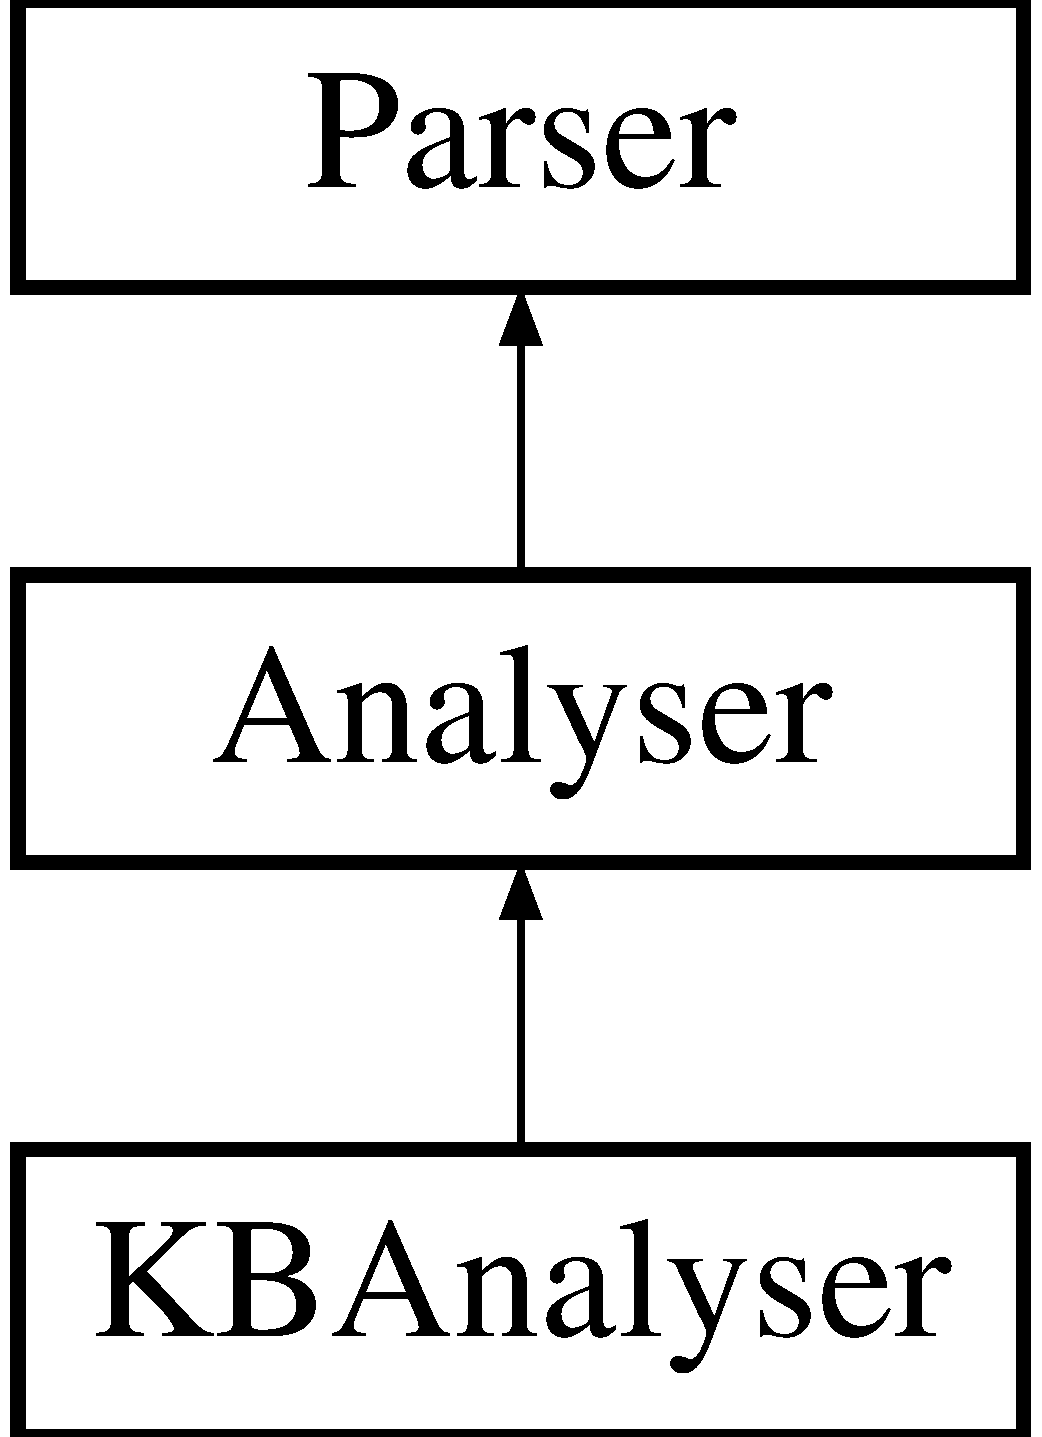
\includegraphics[height=3.000000cm]{classKBAnalyser}
\end{center}
\end{figure}
\subsection*{Public Member Functions}
\begin{DoxyCompactItemize}
\item 
\mbox{\Hypertarget{classKBAnalyser_affef4d1e6d712d466457a2155df4febe}\label{classKBAnalyser_affef4d1e6d712d466457a2155df4febe}} 
\mbox{\hyperlink{classKBAnalyser_affef4d1e6d712d466457a2155df4febe}{K\+B\+Analyser}} ()
\begin{DoxyCompactList}\small\item\em Constructs a new \mbox{\hyperlink{classKBAnalyser}{K\+B\+Analyser}} object. \end{DoxyCompactList}\end{DoxyCompactItemize}
\subsection*{Additional Inherited Members}


\subsection{Detailed Description}
This class represents the analyser responsible for parsing the First Order Logic language. 

The documentation for this class was generated from the following files\+:\begin{DoxyCompactItemize}
\item 
src/\+Agent/\+Knowledge\+Base/\mbox{\hyperlink{KBAnalyser_8h}{K\+B\+Analyser.\+h}}\item 
src/\+Agent/\+Knowledge\+Base/K\+B\+Analyser.\+cpp\end{DoxyCompactItemize}

\hypertarget{classKey}{}\section{Key Class Reference}
\label{classKey}\index{Key@{Key}}
\subsection*{Public Member Functions}
\begin{DoxyCompactItemize}
\item 
\mbox{\Hypertarget{classKey_a36c3d526f01554925ff00ccc03f7c353}\label{classKey_a36c3d526f01554925ff00ccc03f7c353}} 
\mbox{\hyperlink{classKey_a36c3d526f01554925ff00ccc03f7c353}{Key}} (const \mbox{\hyperlink{classString}{String}} \&\mbox{\hyperlink{classKey_a2e5239c4a662635b68778364afd46a96}{name}}, int \mbox{\hyperlink{classKey_ad960b9e4804c3cb039a816811bae4839}{rank}})
\begin{DoxyCompactList}\small\item\em Default constructor. \end{DoxyCompactList}\item 
\mbox{\hyperlink{classDecomp}{Decomp}} $\ast$ \mbox{\hyperlink{classKey_aef5468eea2222639cf3bb839cdd6e6af}{new\+Decomp}} (\mbox{\hyperlink{classString}{String}} script\+Line, \mbox{\hyperlink{classThesaurus}{Thesaurus}} thesaurus)
\item 
\mbox{\hyperlink{classDecomp}{Decomp}} $\ast$ \mbox{\hyperlink{classKey_ad1ee86395985a3b7e6715597c777eeec}{find\+Decomp}} (\mbox{\hyperlink{classString}{String}} str)
\end{DoxyCompactItemize}
\subsection*{Public Attributes}
\begin{DoxyCompactItemize}
\item 
\mbox{\Hypertarget{classKey_a2e5239c4a662635b68778364afd46a96}\label{classKey_a2e5239c4a662635b68778364afd46a96}} 
\mbox{\hyperlink{classString}{String}} \mbox{\hyperlink{classKey_a2e5239c4a662635b68778364afd46a96}{name}}
\begin{DoxyCompactList}\small\item\em Unique key name (identifier) \end{DoxyCompactList}\item 
\mbox{\Hypertarget{classKey_ad960b9e4804c3cb039a816811bae4839}\label{classKey_ad960b9e4804c3cb039a816811bae4839}} 
int \mbox{\hyperlink{classKey_ad960b9e4804c3cb039a816811bae4839}{rank}}
\begin{DoxyCompactList}\small\item\em \mbox{\hyperlink{classKey}{Key}} rank. \end{DoxyCompactList}\item 
\mbox{\Hypertarget{classKey_a48cc30fe4323cd4a0109bdca4c19efd5}\label{classKey_a48cc30fe4323cd4a0109bdca4c19efd5}} 
vector$<$ \mbox{\hyperlink{classDecomp}{Decomp}} $\ast$ $>$ \mbox{\hyperlink{classKey_a48cc30fe4323cd4a0109bdca4c19efd5}{decomp}}
\begin{DoxyCompactList}\small\item\em List of decomposition rules for keyword. \end{DoxyCompactList}\end{DoxyCompactItemize}
\subsection*{Friends}
\begin{DoxyCompactItemize}
\item 
\mbox{\Hypertarget{classKey_a79dc2e19cc4e5d3e4e77d835513e89ca}\label{classKey_a79dc2e19cc4e5d3e4e77d835513e89ca}} 
ostream \& {\bfseries operator$<$$<$} (ostream \&os, const \mbox{\hyperlink{classKey}{Key}} \&key)
\end{DoxyCompactItemize}


\subsection{Member Function Documentation}
\mbox{\Hypertarget{classKey_ad1ee86395985a3b7e6715597c777eeec}\label{classKey_ad1ee86395985a3b7e6715597c777eeec}} 
\index{Key@{Key}!find\+Decomp@{find\+Decomp}}
\index{find\+Decomp@{find\+Decomp}!Key@{Key}}
\subsubsection{\texorpdfstring{find\+Decomp()}{findDecomp()}}
{\footnotesize\ttfamily \mbox{\hyperlink{classDecomp}{Decomp}} $\ast$ Key\+::find\+Decomp (\begin{DoxyParamCaption}\item[{\mbox{\hyperlink{classString}{String}}}]{str }\end{DoxyParamCaption})}

Finds matching decomposition rule for a given string on a keyword using R\+E\+G\+EX. 
\begin{DoxyParams}{Parameters}
{\em str} & Raw string \\
\hline
\end{DoxyParams}
\begin{DoxyReturn}{Returns}
pointer to matching \mbox{\hyperlink{classDecomp}{Decomp}}, or nullptr if no match was found for \mbox{\hyperlink{classKey}{Key}} object. 
\end{DoxyReturn}
\mbox{\Hypertarget{classKey_aef5468eea2222639cf3bb839cdd6e6af}\label{classKey_aef5468eea2222639cf3bb839cdd6e6af}} 
\index{Key@{Key}!new\+Decomp@{new\+Decomp}}
\index{new\+Decomp@{new\+Decomp}!Key@{Key}}
\subsubsection{\texorpdfstring{new\+Decomp()}{newDecomp()}}
{\footnotesize\ttfamily \mbox{\hyperlink{classDecomp}{Decomp}} $\ast$ Key\+::new\+Decomp (\begin{DoxyParamCaption}\item[{\mbox{\hyperlink{classString}{String}}}]{script\+Line,  }\item[{\mbox{\hyperlink{classThesaurus}{Thesaurus}}}]{thesaurus }\end{DoxyParamCaption})}

Creates new decomposition object, adds it to \mbox{\hyperlink{classKey_a48cc30fe4323cd4a0109bdca4c19efd5}{Key.\+decomp}} and links it with the parent \mbox{\hyperlink{classKey}{Key}} object. 
\begin{DoxyParams}{Parameters}
{\em script\+Line} & output string from \mbox{\hyperlink{classScript_a946d037839b4caada09e22a428c8f42e}{Script\+::extract\+Pattern}} \\
\hline
{\em thesaurus} & \mbox{\hyperlink{classScript_afaaa5f986fb3638e31c51231408cfbeb}{Script.\+thes}} \\
\hline
\end{DoxyParams}
\begin{DoxyReturn}{Returns}
pointer to created \mbox{\hyperlink{classDecomp}{Decomp}} 
\end{DoxyReturn}


The documentation for this class was generated from the following files\+:\begin{DoxyCompactItemize}
\item 
src/\+Agent/\+E\+L\+I\+Z\+A/Key.\+h\item 
src/\+Agent/\+E\+L\+I\+Z\+A/Key.\+cpp\end{DoxyCompactItemize}

\hypertarget{classMapper}{}\section{Mapper Class Reference}
\label{classMapper}\index{Mapper@{Mapper}}


Hash table for pre/post script elements.  




{\ttfamily \#include $<$Mapper.\+h$>$}

Inheritance diagram for Mapper\+:\begin{figure}[H]
\begin{center}
\leavevmode
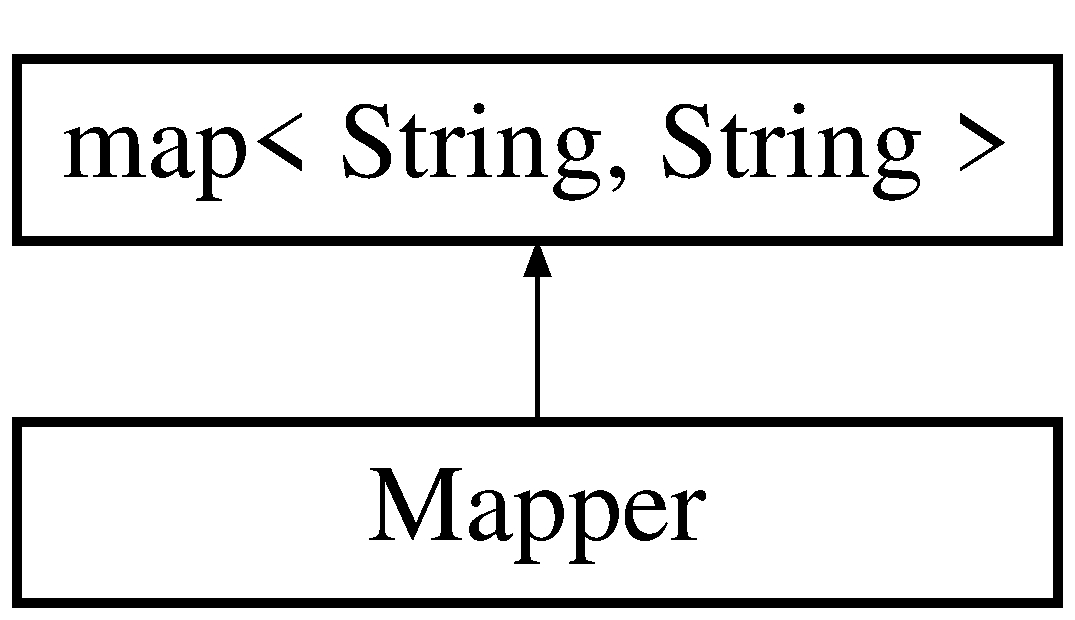
\includegraphics[height=2.000000cm]{classMapper}
\end{center}
\end{figure}
\subsection*{Public Member Functions}
\begin{DoxyCompactItemize}
\item 
void \mbox{\hyperlink{classMapper_aec2d64e739da82af037709cb63d52064}{map}} (\mbox{\hyperlink{classString}{String}} src, \mbox{\hyperlink{classString}{String}} dst)
\item 
\mbox{\hyperlink{classString}{String}} \mbox{\hyperlink{classMapper_a5badcd576626a91fc9b0f76345a64ba8}{translate}} (\mbox{\hyperlink{classString}{String}} sentence)
\end{DoxyCompactItemize}


\subsection{Detailed Description}
Hash table for pre/post script elements. 

\subsection{Member Function Documentation}
\mbox{\Hypertarget{classMapper_aec2d64e739da82af037709cb63d52064}\label{classMapper_aec2d64e739da82af037709cb63d52064}} 
\index{Mapper@{Mapper}!map@{map}}
\index{map@{map}!Mapper@{Mapper}}
\subsubsection{\texorpdfstring{map()}{map()}}
{\footnotesize\ttfamily void Mapper\+::map (\begin{DoxyParamCaption}\item[{\mbox{\hyperlink{classString}{String}}}]{src,  }\item[{\mbox{\hyperlink{classString}{String}}}]{dst }\end{DoxyParamCaption})}

Adds a new element to hash table. 
\begin{DoxyParams}{Parameters}
{\em src} & key \\
\hline
{\em dst} & value \\
\hline
\end{DoxyParams}
\mbox{\Hypertarget{classMapper_a5badcd576626a91fc9b0f76345a64ba8}\label{classMapper_a5badcd576626a91fc9b0f76345a64ba8}} 
\index{Mapper@{Mapper}!translate@{translate}}
\index{translate@{translate}!Mapper@{Mapper}}
\subsubsection{\texorpdfstring{translate()}{translate()}}
{\footnotesize\ttfamily \mbox{\hyperlink{classString}{String}} Mapper\+::translate (\begin{DoxyParamCaption}\item[{\mbox{\hyperlink{classString}{String}}}]{sentence }\end{DoxyParamCaption})}

Translates keywords in a sentence into their values from the hash table. 
\begin{DoxyParams}{Parameters}
{\em sentence} & string of words \\
\hline
\end{DoxyParams}
\begin{DoxyReturn}{Returns}
Translated sentence 
\end{DoxyReturn}


The documentation for this class was generated from the following files\+:\begin{DoxyCompactItemize}
\item 
src/\+Agent/\+E\+L\+I\+Z\+A/Mapper.\+h\item 
src/\+Agent/\+E\+L\+I\+Z\+A/Mapper.\+cpp\end{DoxyCompactItemize}

\hypertarget{classMemory}{}\section{Memory Class Reference}
\label{classMemory}\index{Memory@{Memory}}


F\+I\+FO stack of \mbox{\hyperlink{classReasmb}{Reasmb}} objects.  




{\ttfamily \#include $<$Memory.\+h$>$}

Inheritance diagram for Memory\+:\begin{figure}[H]
\begin{center}
\leavevmode
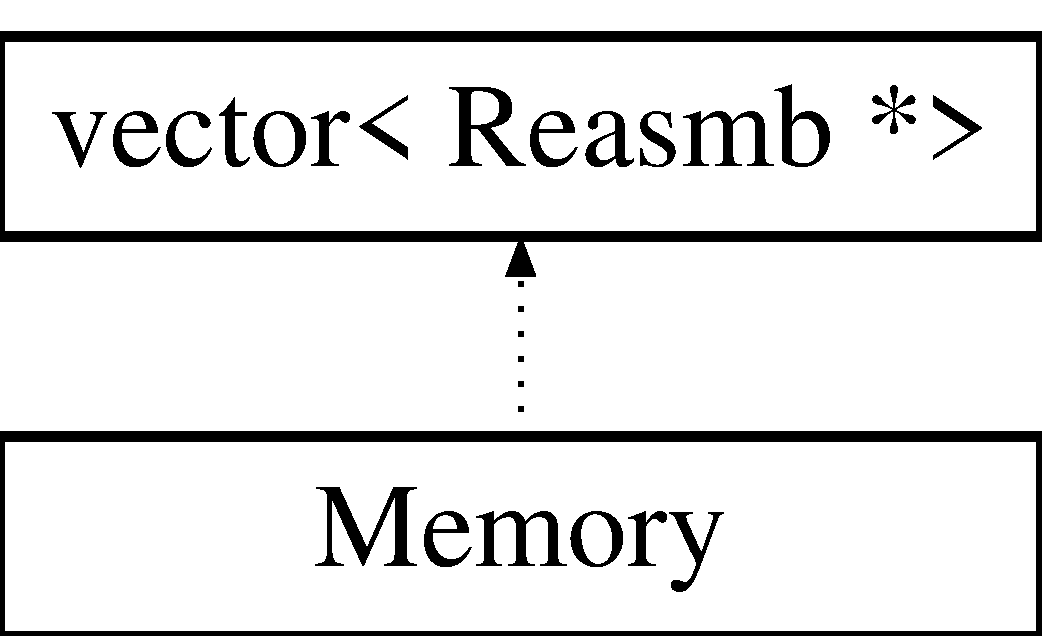
\includegraphics[height=2.000000cm]{classMemory}
\end{center}
\end{figure}
\subsection*{Public Member Functions}
\begin{DoxyCompactItemize}
\item 
\mbox{\Hypertarget{classMemory_a69385c2f0b8711506d38883bdcbdb7ba}\label{classMemory_a69385c2f0b8711506d38883bdcbdb7ba}} 
void \mbox{\hyperlink{classMemory_a69385c2f0b8711506d38883bdcbdb7ba}{save}} (\mbox{\hyperlink{classReasmb}{Reasmb}} $\ast$)
\begin{DoxyCompactList}\small\item\em Saves new reassembly rule in memory. \end{DoxyCompactList}\item 
\mbox{\Hypertarget{classMemory_ae10852b620d16e695add6890f9dc298d}\label{classMemory_ae10852b620d16e695add6890f9dc298d}} 
\mbox{\hyperlink{classReasmb}{Reasmb}} $\ast$ \mbox{\hyperlink{classMemory_ae10852b620d16e695add6890f9dc298d}{pop}} ()
\begin{DoxyCompactList}\small\item\em Pops first reassembly rule from memory. \end{DoxyCompactList}\end{DoxyCompactItemize}
\subsection*{Private Attributes}
\begin{DoxyCompactItemize}
\item 
\mbox{\Hypertarget{classMemory_af3c95c183e92e91899dc677c683f2b66}\label{classMemory_af3c95c183e92e91899dc677c683f2b66}} 
size\+\_\+t \mbox{\hyperlink{classMemory_af3c95c183e92e91899dc677c683f2b66}{max}} = 20
\begin{DoxyCompactList}\small\item\em \mbox{\hyperlink{classMemory}{Memory}} capacity. \end{DoxyCompactList}\end{DoxyCompactItemize}


\subsection{Detailed Description}
F\+I\+FO stack of \mbox{\hyperlink{classReasmb}{Reasmb}} objects. 

The documentation for this class was generated from the following files\+:\begin{DoxyCompactItemize}
\item 
src/\+Agent/\+E\+L\+I\+Z\+A/Memory.\+h\item 
src/\+Agent/\+E\+L\+I\+Z\+A/Memory.\+cpp\end{DoxyCompactItemize}

\hypertarget{classParser}{}\section{Parser Class Reference}
\label{classParser}\index{Parser@{Parser}}


Parses source file into appropriate data types.  




{\ttfamily \#include $<$Parser.\+h$>$}

Inheritance diagram for Parser\+:\begin{figure}[H]
\begin{center}
\leavevmode
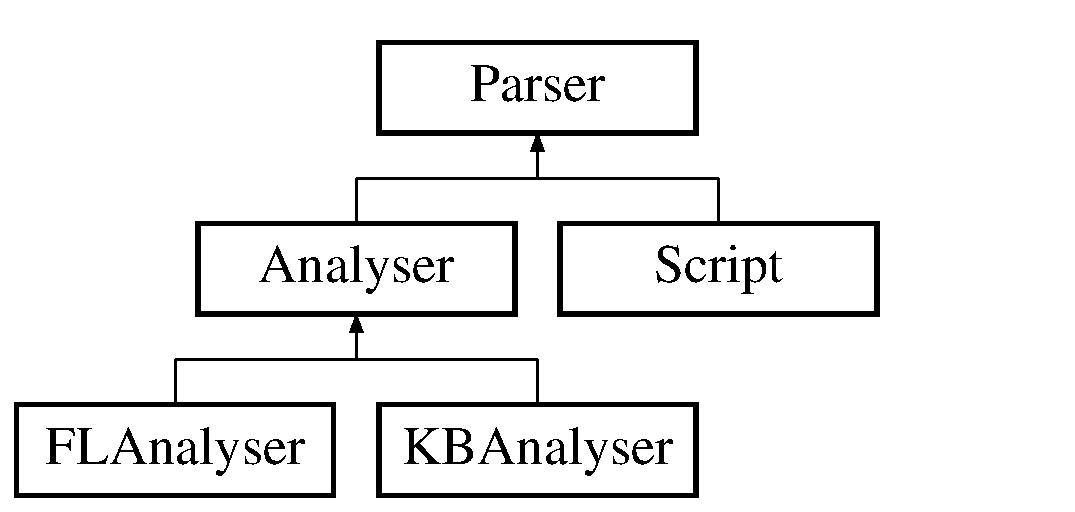
\includegraphics[height=3.000000cm]{classParser}
\end{center}
\end{figure}
\subsection*{Public Member Functions}
\begin{DoxyCompactItemize}
\item 
\mbox{\hyperlink{classParser_a0561a18255812c46ece89f199ce337a8}{Parser}} (\mbox{\hyperlink{classString}{String}} \mbox{\hyperlink{classParser_a9af73d63c4685837209f362dababa554}{source\+Path}})
\end{DoxyCompactItemize}
\subsection*{Public Attributes}
\begin{DoxyCompactItemize}
\item 
\mbox{\Hypertarget{classParser_a9af73d63c4685837209f362dababa554}\label{classParser_a9af73d63c4685837209f362dababa554}} 
\mbox{\hyperlink{classString}{String}} \mbox{\hyperlink{classParser_a9af73d63c4685837209f362dababa554}{source\+Path}}
\begin{DoxyCompactList}\small\item\em Source file path. \end{DoxyCompactList}\end{DoxyCompactItemize}
\subsection*{Protected Member Functions}
\begin{DoxyCompactItemize}
\item 
virtual void \mbox{\hyperlink{classParser_a1df9aa58be0f4027a39277d78b870195}{parse}} ()=0
\end{DoxyCompactItemize}


\subsection{Detailed Description}
Parses source file into appropriate data types. 

\subsection{Constructor \& Destructor Documentation}
\mbox{\Hypertarget{classParser_a0561a18255812c46ece89f199ce337a8}\label{classParser_a0561a18255812c46ece89f199ce337a8}} 
\index{Parser@{Parser}!Parser@{Parser}}
\index{Parser@{Parser}!Parser@{Parser}}
\subsubsection{\texorpdfstring{Parser()}{Parser()}}
{\footnotesize\ttfamily Parser\+::\+Parser (\begin{DoxyParamCaption}\item[{\mbox{\hyperlink{classString}{String}}}]{source\+Path }\end{DoxyParamCaption})}

\mbox{\hyperlink{classParser}{Parser}} default constructor. 
\begin{DoxyParams}{Parameters}
{\em source\+Path} & source file path \\
\hline
\end{DoxyParams}


\subsection{Member Function Documentation}
\mbox{\Hypertarget{classParser_a1df9aa58be0f4027a39277d78b870195}\label{classParser_a1df9aa58be0f4027a39277d78b870195}} 
\index{Parser@{Parser}!parse@{parse}}
\index{parse@{parse}!Parser@{Parser}}
\subsubsection{\texorpdfstring{parse()}{parse()}}
{\footnotesize\ttfamily virtual void Parser\+::parse (\begin{DoxyParamCaption}{ }\end{DoxyParamCaption})\hspace{0.3cm}{\ttfamily [protected]}, {\ttfamily [pure virtual]}}

Called by constructor to parse data from source file. 

Implemented in \mbox{\hyperlink{classScript_a4bb2f5d77aed84a9f0dc9298894abd1c}{Script}}.



The documentation for this class was generated from the following files\+:\begin{DoxyCompactItemize}
\item 
src/\+Agent/Parser.\+h\item 
src/\+Agent/Parser.\+cpp\end{DoxyCompactItemize}

\hypertarget{classPercept}{}\section{Percept Class Reference}
\label{classPercept}\index{Percept@{Percept}}


This class represents a perception received by the agent (which is of an exclusive text form in our case).  




{\ttfamily \#include $<$Percept.\+h$>$}

\subsection*{Public Member Functions}
\begin{DoxyCompactItemize}
\item 
vector$<$ \mbox{\hyperlink{classSentence}{Sentence}} $>$ \mbox{\hyperlink{classPercept_a3912d5efafea356d07436b791a97684c}{make\+Percept\+Sentence}} (\mbox{\hyperlink{classPercept}{Percept}} p)
\begin{DoxyCompactList}\small\item\em This function turns a percept into a logical sentence. \end{DoxyCompactList}\end{DoxyCompactItemize}
\subsection*{Public Attributes}
\begin{DoxyCompactItemize}
\item 
int \mbox{\hyperlink{classPercept_a87baa8b4903f43f03a86430185a36840}{id}}
\end{DoxyCompactItemize}
\subsection*{Private Attributes}
\begin{DoxyCompactItemize}
\item 
\mbox{\hyperlink{classString}{String}} \mbox{\hyperlink{classPercept_acd9d577a5dce1064a78d87f26ec10be7}{string\+\_\+feed}}
\item 
vector$<$ \mbox{\hyperlink{classSentence}{Sentence}} $>$ \mbox{\hyperlink{classPercept_a4b92db8d220627cd58a61eb8f6d1faa6}{logic\+\_\+feed}}
\end{DoxyCompactItemize}


\subsection{Detailed Description}
This class represents a perception received by the agent (which is of an exclusive text form in our case). 

\subsection{Member Function Documentation}
\mbox{\Hypertarget{classPercept_a3912d5efafea356d07436b791a97684c}\label{classPercept_a3912d5efafea356d07436b791a97684c}} 
\index{Percept@{Percept}!make\+Percept\+Sentence@{make\+Percept\+Sentence}}
\index{make\+Percept\+Sentence@{make\+Percept\+Sentence}!Percept@{Percept}}
\subsubsection{\texorpdfstring{make\+Percept\+Sentence()}{makePerceptSentence()}}
{\footnotesize\ttfamily vector$<$ \mbox{\hyperlink{classSentence}{Sentence}} $>$ Percept\+::make\+Percept\+Sentence (\begin{DoxyParamCaption}\item[{\mbox{\hyperlink{classPercept}{Percept}}}]{p }\end{DoxyParamCaption})}



This function turns a percept into a logical sentence. 


\begin{DoxyParams}{Parameters}
{\em p} & The percepts to be converted. \\
\hline
\end{DoxyParams}
\begin{DoxyReturn}{Returns}
A logical sentence. 
\end{DoxyReturn}


\subsection{Member Data Documentation}
\mbox{\Hypertarget{classPercept_a87baa8b4903f43f03a86430185a36840}\label{classPercept_a87baa8b4903f43f03a86430185a36840}} 
\index{Percept@{Percept}!id@{id}}
\index{id@{id}!Percept@{Percept}}
\subsubsection{\texorpdfstring{id}{id}}
{\footnotesize\ttfamily int Percept\+::id}

Each percept bears a unique number. \mbox{\Hypertarget{classPercept_a4b92db8d220627cd58a61eb8f6d1faa6}\label{classPercept_a4b92db8d220627cd58a61eb8f6d1faa6}} 
\index{Percept@{Percept}!logic\+\_\+feed@{logic\+\_\+feed}}
\index{logic\+\_\+feed@{logic\+\_\+feed}!Percept@{Percept}}
\subsubsection{\texorpdfstring{logic\+\_\+feed}{logic\_feed}}
{\footnotesize\ttfamily vector$<$\mbox{\hyperlink{classSentence}{Sentence}}$>$ Percept\+::logic\+\_\+feed\hspace{0.3cm}{\ttfamily [private]}}

Represents the logical form of a percept. \mbox{\Hypertarget{classPercept_acd9d577a5dce1064a78d87f26ec10be7}\label{classPercept_acd9d577a5dce1064a78d87f26ec10be7}} 
\index{Percept@{Percept}!string\+\_\+feed@{string\+\_\+feed}}
\index{string\+\_\+feed@{string\+\_\+feed}!Percept@{Percept}}
\subsubsection{\texorpdfstring{string\+\_\+feed}{string\_feed}}
{\footnotesize\ttfamily \mbox{\hyperlink{classString}{String}} Percept\+::string\+\_\+feed\hspace{0.3cm}{\ttfamily [private]}}

Represents the text form of a percept. 

The documentation for this class was generated from the following files\+:\begin{DoxyCompactItemize}
\item 
src/\+Agent/\+Knowledge\+Base/\mbox{\hyperlink{Percept_8h}{Percept.\+h}}\item 
src/\+Agent/\+Knowledge\+Base/Percept.\+cpp\end{DoxyCompactItemize}

\hypertarget{classReasmb}{}\section{Reasmb Class Reference}
\label{classReasmb}\index{Reasmb@{Reasmb}}


Reassembly rule for decomposed sentence.  




{\ttfamily \#include $<$Reasmb.\+h$>$}

\subsection*{Public Member Functions}
\begin{DoxyCompactItemize}
\item 
\mbox{\Hypertarget{classReasmb_a3b2f5458d8810917c76cfaac15b749d4}\label{classReasmb_a3b2f5458d8810917c76cfaac15b749d4}} 
{\bfseries Reasmb} (\mbox{\hyperlink{classDecomp}{Decomp}} $\ast$\mbox{\hyperlink{classReasmb_a70b89635a2cc4f04cd30ec0bcb0bd0bf}{decomp}}, const \mbox{\hyperlink{classString}{String}} \&\mbox{\hyperlink{classReasmb_a5f6b1b32f233f3dc7222f324791337c2}{rule}})
\item 
\mbox{\hyperlink{classString}{String}} \mbox{\hyperlink{classReasmb_abba1a0d8940231ac3e9ce7fd39173eb4}{reassemble}} (vector$<$ \mbox{\hyperlink{classString}{String}} $>$ matches)
\end{DoxyCompactItemize}
\subsection*{Public Attributes}
\begin{DoxyCompactItemize}
\item 
\mbox{\Hypertarget{classReasmb_a70b89635a2cc4f04cd30ec0bcb0bd0bf}\label{classReasmb_a70b89635a2cc4f04cd30ec0bcb0bd0bf}} 
\mbox{\hyperlink{classDecomp}{Decomp}} $\ast$ \mbox{\hyperlink{classReasmb_a70b89635a2cc4f04cd30ec0bcb0bd0bf}{decomp}}
\begin{DoxyCompactList}\small\item\em Pointer to parent decomposition rule. \end{DoxyCompactList}\item 
\mbox{\Hypertarget{classReasmb_a5f6b1b32f233f3dc7222f324791337c2}\label{classReasmb_a5f6b1b32f233f3dc7222f324791337c2}} 
\mbox{\hyperlink{classString}{String}} \mbox{\hyperlink{classReasmb_a5f6b1b32f233f3dc7222f324791337c2}{rule}}
\begin{DoxyCompactList}\small\item\em Reassembly rule pattern. \end{DoxyCompactList}\end{DoxyCompactItemize}
\subsection*{Friends}
\begin{DoxyCompactItemize}
\item 
\mbox{\Hypertarget{classReasmb_a705525beb8fb25cb1d4b9ba89b055e67}\label{classReasmb_a705525beb8fb25cb1d4b9ba89b055e67}} 
ostream \& {\bfseries operator$<$$<$} (ostream \&os, const \mbox{\hyperlink{classReasmb}{Reasmb}} \&reasmb)
\end{DoxyCompactItemize}


\subsection{Detailed Description}
Reassembly rule for decomposed sentence. 

\subsection{Member Function Documentation}
\mbox{\Hypertarget{classReasmb_abba1a0d8940231ac3e9ce7fd39173eb4}\label{classReasmb_abba1a0d8940231ac3e9ce7fd39173eb4}} 
\index{Reasmb@{Reasmb}!reassemble@{reassemble}}
\index{reassemble@{reassemble}!Reasmb@{Reasmb}}
\subsubsection{\texorpdfstring{reassemble()}{reassemble()}}
{\footnotesize\ttfamily \mbox{\hyperlink{classString}{String}} Reasmb\+::reassemble (\begin{DoxyParamCaption}\item[{vector$<$ \mbox{\hyperlink{classString}{String}} $>$}]{matches }\end{DoxyParamCaption})}

Reassembles sentence from matching expressions. 
\begin{DoxyParams}{Parameters}
{\em matches} & output of \mbox{\hyperlink{classDecomp_a5778e75423e33df37fe2e41157d3bc03}{Decomp\+::decompose}} \\
\hline
\end{DoxyParams}
\begin{DoxyReturn}{Returns}
reassembled response 
\end{DoxyReturn}


The documentation for this class was generated from the following files\+:\begin{DoxyCompactItemize}
\item 
src/\+Agent/\+E\+L\+I\+Z\+A/Reasmb.\+h\item 
src/\+Agent/\+E\+L\+I\+Z\+A/Reasmb.\+cpp\end{DoxyCompactItemize}

\hypertarget{classScript}{}\section{Script Class Reference}
\label{classScript}\index{Script@{Script}}
Inheritance diagram for Script\+:\begin{figure}[H]
\begin{center}
\leavevmode
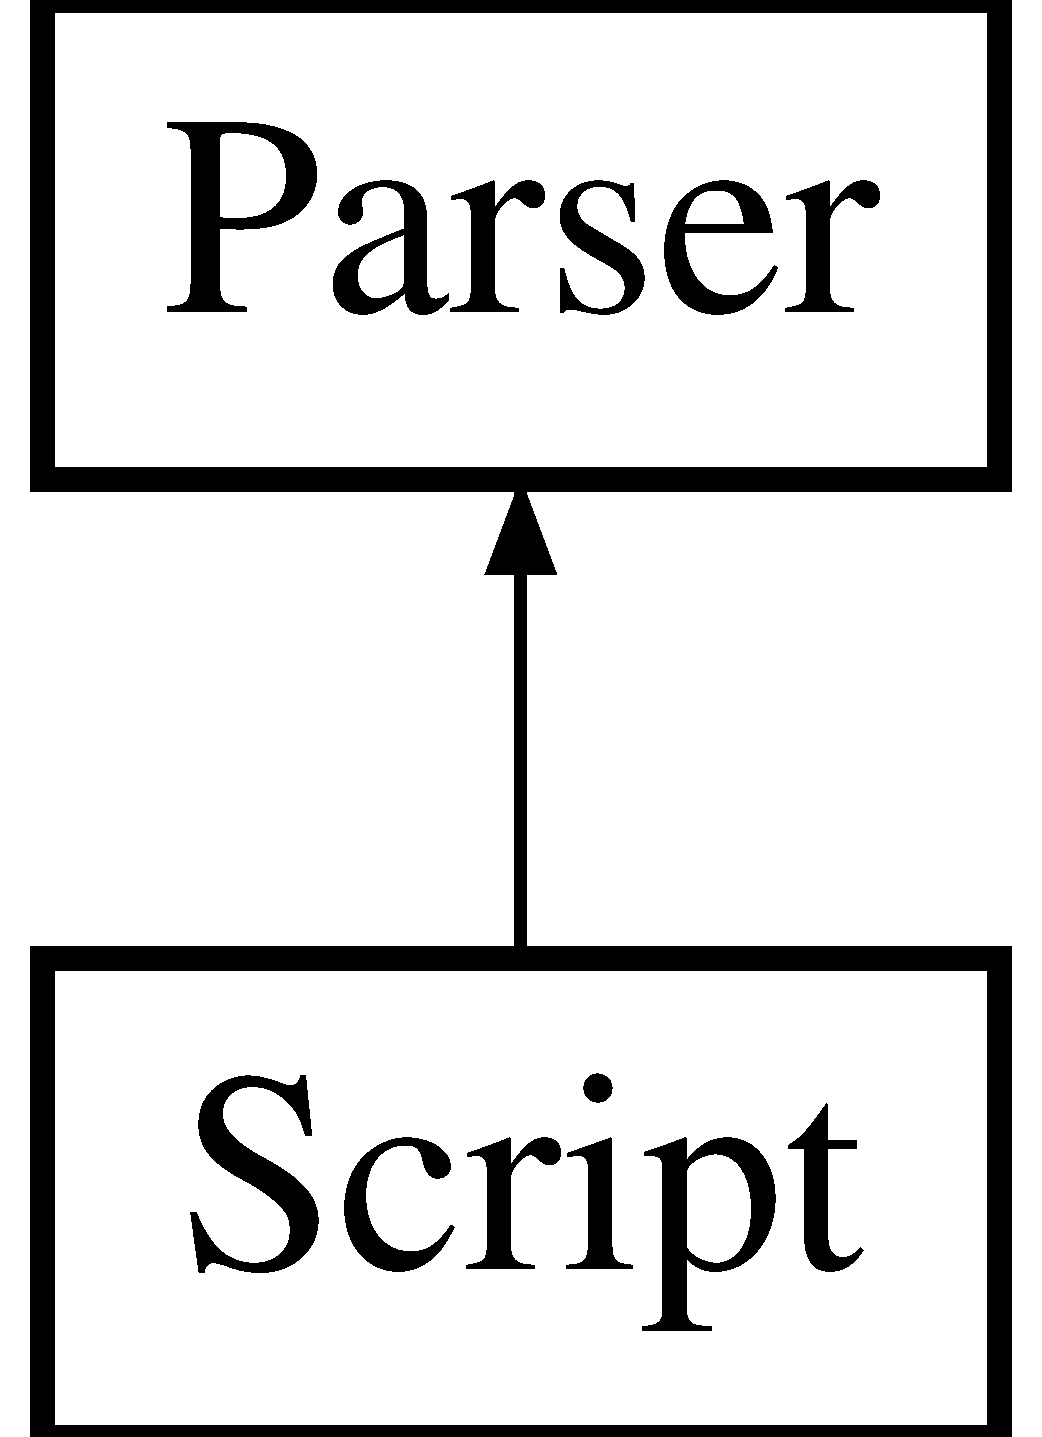
\includegraphics[height=2.000000cm]{classScript}
\end{center}
\end{figure}
\subsection*{Public Member Functions}
\begin{DoxyCompactItemize}
\item 
\mbox{\Hypertarget{classScript_ad9e14ce089abb34c1acb97fcfd161b54}\label{classScript_ad9e14ce089abb34c1acb97fcfd161b54}} 
{\bfseries Script} (const \mbox{\hyperlink{classString}{String}} \&\mbox{\hyperlink{classParser_a9af73d63c4685837209f362dababa554}{source\+Path}})
\item 
\mbox{\hyperlink{classString}{String}} \mbox{\hyperlink{classScript_af94dd912c6276f5130d13740d775200c}{pre\+\_\+translate}} (\mbox{\hyperlink{classString}{String}} str)
\item 
\mbox{\hyperlink{classString}{String}} \mbox{\hyperlink{classScript_a754cc2f448013d0a3b400088e460fbe4}{post\+\_\+translate}} (\mbox{\hyperlink{classString}{String}} str)
\item 
\mbox{\hyperlink{classKey}{Key}} $\ast$ \mbox{\hyperlink{classScript_a027acbd1cfa4440c9eb51a2b6c91c6a0}{get\+Key}} (\mbox{\hyperlink{classString}{String}} word)
\end{DoxyCompactItemize}
\subsection*{Public Attributes}
\begin{DoxyCompactItemize}
\item 
\mbox{\Hypertarget{classScript_a179b6b4f3ac3c7d8f4a4dd59ab7c262c}\label{classScript_a179b6b4f3ac3c7d8f4a4dd59ab7c262c}} 
\mbox{\hyperlink{classString}{String}} \mbox{\hyperlink{classScript_a179b6b4f3ac3c7d8f4a4dd59ab7c262c}{initial}}
\begin{DoxyCompactList}\small\item\em Initial string to greet user. \end{DoxyCompactList}\item 
\mbox{\Hypertarget{classScript_a3918303573708a77fe61c2ec91865dc9}\label{classScript_a3918303573708a77fe61c2ec91865dc9}} 
\mbox{\hyperlink{classString}{String}} \mbox{\hyperlink{classScript_a3918303573708a77fe61c2ec91865dc9}{final}}
\begin{DoxyCompactList}\small\item\em Final string to bid farewell to user. \end{DoxyCompactList}\item 
\mbox{\Hypertarget{classScript_ab338df3426a5f488be94ec6c15393ba6}\label{classScript_ab338df3426a5f488be94ec6c15393ba6}} 
\mbox{\hyperlink{classMapper}{Mapper}} \mbox{\hyperlink{classScript_ab338df3426a5f488be94ec6c15393ba6}{pre}}
\begin{DoxyCompactList}\small\item\em Pre-\/processing map database. \end{DoxyCompactList}\item 
\mbox{\Hypertarget{classScript_ac73831210ecd442bbeafbd9a496bb042}\label{classScript_ac73831210ecd442bbeafbd9a496bb042}} 
\mbox{\hyperlink{classMapper}{Mapper}} \mbox{\hyperlink{classScript_ac73831210ecd442bbeafbd9a496bb042}{post}}
\begin{DoxyCompactList}\small\item\em Post-\/processing map database. \end{DoxyCompactList}\item 
\mbox{\Hypertarget{classScript_ad1fcd3868d74927bd60118f0e4eaf574}\label{classScript_ad1fcd3868d74927bd60118f0e4eaf574}} 
vector$<$ \mbox{\hyperlink{classKey}{Key}} $\ast$ $>$ \mbox{\hyperlink{classScript_ad1fcd3868d74927bd60118f0e4eaf574}{keys}}
\begin{DoxyCompactList}\small\item\em List of keywords in database. \end{DoxyCompactList}\item 
\mbox{\Hypertarget{classScript_a187f8b939336ed6f1a5b7cf44526eacf}\label{classScript_a187f8b939336ed6f1a5b7cf44526eacf}} 
vector$<$ \mbox{\hyperlink{classString}{String}} $>$ \mbox{\hyperlink{classScript_a187f8b939336ed6f1a5b7cf44526eacf}{quit}}
\begin{DoxyCompactList}\small\item\em List of strings that the user can enter to end the conversation. \end{DoxyCompactList}\item 
\mbox{\Hypertarget{classScript_afaaa5f986fb3638e31c51231408cfbeb}\label{classScript_afaaa5f986fb3638e31c51231408cfbeb}} 
\mbox{\hyperlink{classThesaurus}{Thesaurus}} \mbox{\hyperlink{classScript_afaaa5f986fb3638e31c51231408cfbeb}{thes}}
\begin{DoxyCompactList}\small\item\em \mbox{\hyperlink{classThesaurus}{Thesaurus}} (list of synonyms) in database. \end{DoxyCompactList}\end{DoxyCompactItemize}
\subsection*{Private Member Functions}
\begin{DoxyCompactItemize}
\item 
void \mbox{\hyperlink{classScript_a4bb2f5d77aed84a9f0dc9298894abd1c}{parse}} () override
\item 
\mbox{\hyperlink{classString}{String}} \mbox{\hyperlink{classScript_a946d037839b4caada09e22a428c8f42e}{extract\+Pattern}} (\mbox{\hyperlink{classString}{String}} line, \mbox{\hyperlink{classString}{String}} key)
\item 
\mbox{\hyperlink{classKey}{Key}} $\ast$ \mbox{\hyperlink{classScript_a5edeec2fa0d7e46e0795715810a031d8}{new\+Key}} (\mbox{\hyperlink{classString}{String}} script\+Line)
\end{DoxyCompactItemize}
\subsection*{Friends}
\begin{DoxyCompactItemize}
\item 
\mbox{\Hypertarget{classScript_a28fbd10cd3ac6e431b96d64453c23dec}\label{classScript_a28fbd10cd3ac6e431b96d64453c23dec}} 
ostream \& {\bfseries operator$<$$<$} (ostream \&os, const \mbox{\hyperlink{classScript}{Script}} \&parser)
\end{DoxyCompactItemize}
\subsection*{Additional Inherited Members}


\subsection{Member Function Documentation}
\mbox{\Hypertarget{classScript_a946d037839b4caada09e22a428c8f42e}\label{classScript_a946d037839b4caada09e22a428c8f42e}} 
\index{Script@{Script}!extract\+Pattern@{extract\+Pattern}}
\index{extract\+Pattern@{extract\+Pattern}!Script@{Script}}
\subsubsection{\texorpdfstring{extract\+Pattern()}{extractPattern()}}
{\footnotesize\ttfamily \mbox{\hyperlink{classString}{String}} Script\+::extract\+Pattern (\begin{DoxyParamCaption}\item[{\mbox{\hyperlink{classString}{String}}}]{line,  }\item[{\mbox{\hyperlink{classString}{String}}}]{key }\end{DoxyParamCaption})\hspace{0.3cm}{\ttfamily [private]}}

Extracts pattern definition from a line from the script file. 
\begin{DoxyParams}{Parameters}
{\em line} & line from script file \\
\hline
{\em key} & script element identifier key \\
\hline
\end{DoxyParams}
\begin{DoxyReturn}{Returns}
extracted pattern if the given key is in line, an empty string otherwise.
\end{DoxyReturn}
Usage example\+: 
\begin{DoxyCode}
line = \textcolor{stringliteral}{"reasmb: Do you feel strongly about discussing such things ?"};
pattern = \mbox{\hyperlink{classScript_a946d037839b4caada09e22a428c8f42e}{extractPattern}}(line, \textcolor{stringliteral}{"reasmb"}); \textcolor{comment}{// pattern = "Do you feel strongly about discussing
       such things ?"}
pattern = \mbox{\hyperlink{classScript_a946d037839b4caada09e22a428c8f42e}{extractPattern}}(line, \textcolor{stringliteral}{"decomp"}); \textcolor{comment}{// pattern = ""}
\end{DoxyCode}
 \mbox{\Hypertarget{classScript_a027acbd1cfa4440c9eb51a2b6c91c6a0}\label{classScript_a027acbd1cfa4440c9eb51a2b6c91c6a0}} 
\index{Script@{Script}!get\+Key@{get\+Key}}
\index{get\+Key@{get\+Key}!Script@{Script}}
\subsubsection{\texorpdfstring{get\+Key()}{getKey()}}
{\footnotesize\ttfamily \mbox{\hyperlink{classKey}{Key}} $\ast$ Script\+::get\+Key (\begin{DoxyParamCaption}\item[{\mbox{\hyperlink{classString}{String}}}]{word }\end{DoxyParamCaption})}

Finds keyword in database 
\begin{DoxyParams}{Parameters}
{\em word} & given word \\
\hline
\end{DoxyParams}
\begin{DoxyReturn}{Returns}
associated \mbox{\hyperlink{classKey}{Key}} object 
\end{DoxyReturn}
\mbox{\Hypertarget{classScript_a5edeec2fa0d7e46e0795715810a031d8}\label{classScript_a5edeec2fa0d7e46e0795715810a031d8}} 
\index{Script@{Script}!new\+Key@{new\+Key}}
\index{new\+Key@{new\+Key}!Script@{Script}}
\subsubsection{\texorpdfstring{new\+Key()}{newKey()}}
{\footnotesize\ttfamily \mbox{\hyperlink{classKey}{Key}} $\ast$ Script\+::new\+Key (\begin{DoxyParamCaption}\item[{\mbox{\hyperlink{classString}{String}}}]{script\+Line }\end{DoxyParamCaption})\hspace{0.3cm}{\ttfamily [private]}}

Creates new \mbox{\hyperlink{classKey}{Key}} object and adds it to \mbox{\hyperlink{classScript_ad1fcd3868d74927bd60118f0e4eaf574}{Script.\+keys}} 
\begin{DoxyParams}{Parameters}
{\em script\+Line} & output string from \mbox{\hyperlink{classScript_a946d037839b4caada09e22a428c8f42e}{Script\+::extract\+Pattern}} \\
\hline
\end{DoxyParams}
\begin{DoxyReturn}{Returns}
pointer to created \mbox{\hyperlink{classKey}{Key}} 
\end{DoxyReturn}
\mbox{\Hypertarget{classScript_a4bb2f5d77aed84a9f0dc9298894abd1c}\label{classScript_a4bb2f5d77aed84a9f0dc9298894abd1c}} 
\index{Script@{Script}!parse@{parse}}
\index{parse@{parse}!Script@{Script}}
\subsubsection{\texorpdfstring{parse()}{parse()}}
{\footnotesize\ttfamily void Script\+::parse (\begin{DoxyParamCaption}{ }\end{DoxyParamCaption})\hspace{0.3cm}{\ttfamily [override]}, {\ttfamily [private]}, {\ttfamily [virtual]}}

Called by constructor to parse data from source file. 

Implements \mbox{\hyperlink{classParser_a1df9aa58be0f4027a39277d78b870195}{Parser}}.

\mbox{\Hypertarget{classScript_a754cc2f448013d0a3b400088e460fbe4}\label{classScript_a754cc2f448013d0a3b400088e460fbe4}} 
\index{Script@{Script}!post\+\_\+translate@{post\+\_\+translate}}
\index{post\+\_\+translate@{post\+\_\+translate}!Script@{Script}}
\subsubsection{\texorpdfstring{post\+\_\+translate()}{post\_translate()}}
{\footnotesize\ttfamily \mbox{\hyperlink{classString}{String}} Script\+::post\+\_\+translate (\begin{DoxyParamCaption}\item[{\mbox{\hyperlink{classString}{String}}}]{str }\end{DoxyParamCaption})}

Post-\/translates output string 
\begin{DoxyParams}{Parameters}
{\em output} & raw output string \\
\hline
\end{DoxyParams}
\begin{DoxyReturn}{Returns}
processed output 
\end{DoxyReturn}
\mbox{\Hypertarget{classScript_af94dd912c6276f5130d13740d775200c}\label{classScript_af94dd912c6276f5130d13740d775200c}} 
\index{Script@{Script}!pre\+\_\+translate@{pre\+\_\+translate}}
\index{pre\+\_\+translate@{pre\+\_\+translate}!Script@{Script}}
\subsubsection{\texorpdfstring{pre\+\_\+translate()}{pre\_translate()}}
{\footnotesize\ttfamily \mbox{\hyperlink{classString}{String}} Script\+::pre\+\_\+translate (\begin{DoxyParamCaption}\item[{\mbox{\hyperlink{classString}{String}}}]{str }\end{DoxyParamCaption})}

Pre-\/translates input string 
\begin{DoxyParams}{Parameters}
{\em input} & user\textquotesingle{}s raw input \\
\hline
\end{DoxyParams}
\begin{DoxyReturn}{Returns}
processed input 
\end{DoxyReturn}


The documentation for this class was generated from the following files\+:\begin{DoxyCompactItemize}
\item 
src/\+Agent/\+E\+L\+I\+Z\+A/Script.\+h\item 
src/\+Agent/\+E\+L\+I\+Z\+A/Script.\+cpp\end{DoxyCompactItemize}

\hypertarget{classSentence}{}\section{Sentence Class Reference}
\label{classSentence}\index{Sentence@{Sentence}}


Class representing a sentence.  




{\ttfamily \#include $<$Sentence.\+h$>$}



\subsection{Detailed Description}
Class representing a sentence. 

The documentation for this class was generated from the following file\+:\begin{DoxyCompactItemize}
\item 
src/\+Agent/\+Knowledge\+Base/\mbox{\hyperlink{Sentence_8h}{Sentence.\+h}}\end{DoxyCompactItemize}

\hypertarget{classString}{}\section{String Class Reference}
\label{classString}\index{String@{String}}


An extended string class with useful methods.  




{\ttfamily \#include $<$String.\+h$>$}

Inheritance diagram for String\+:\begin{figure}[H]
\begin{center}
\leavevmode
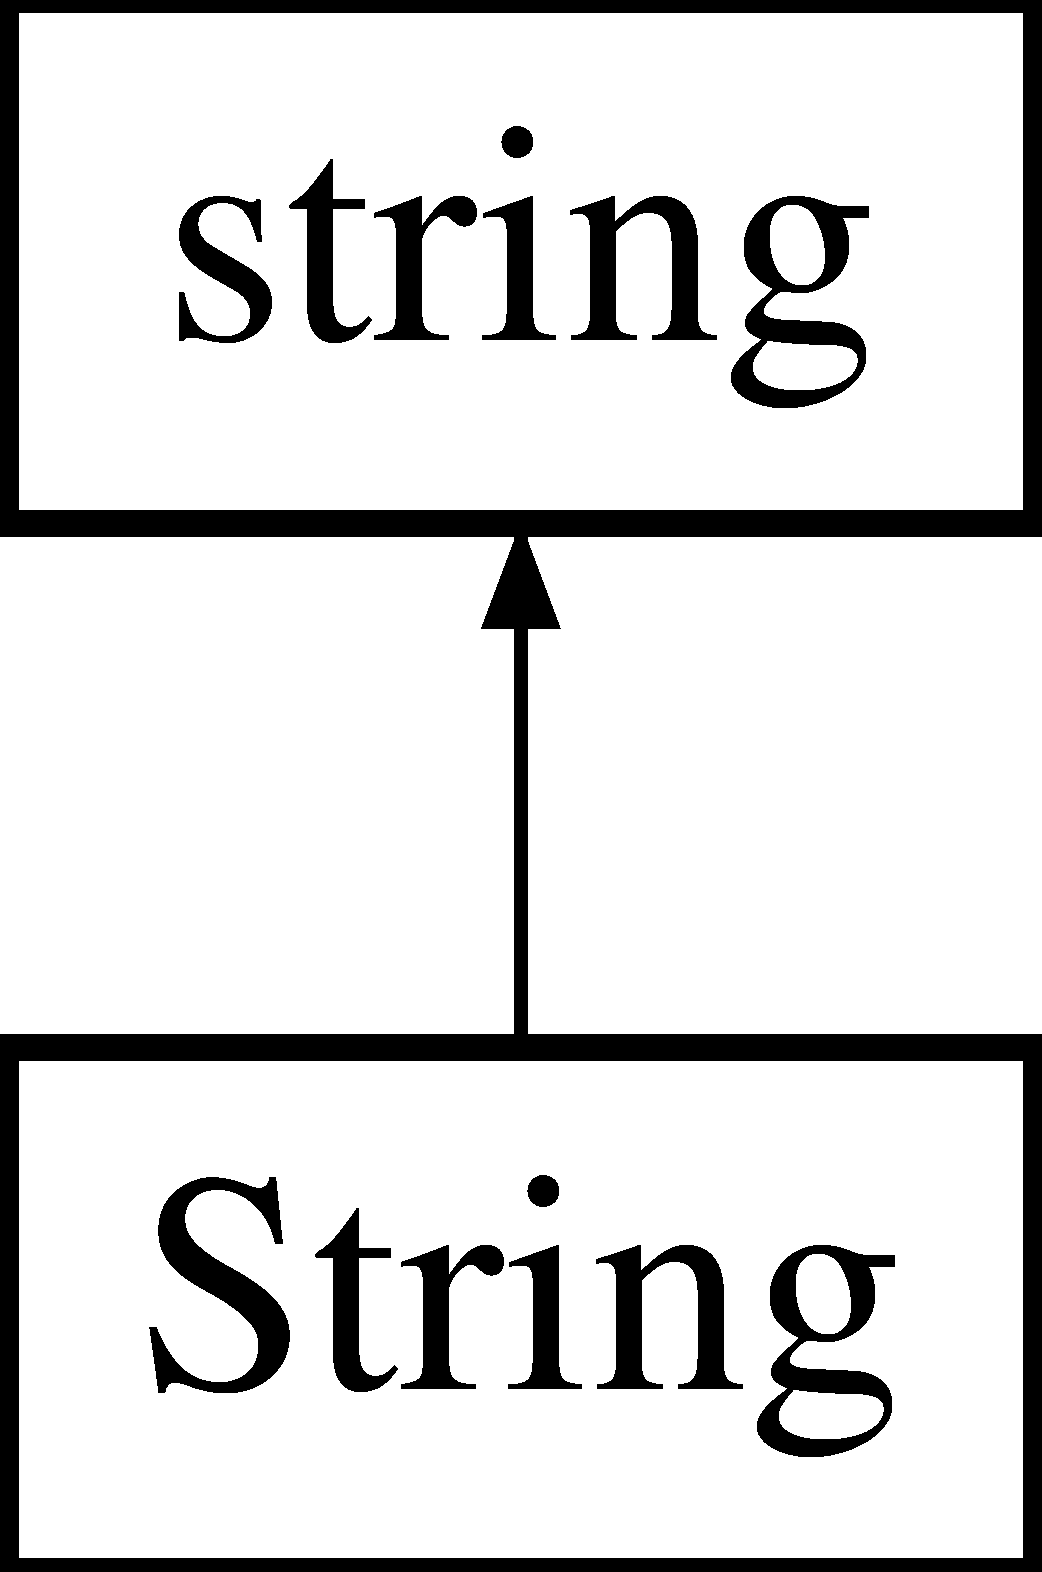
\includegraphics[height=2.000000cm]{classString}
\end{center}
\end{figure}
\subsection*{Public Member Functions}
\begin{DoxyCompactItemize}
\item 
\mbox{\Hypertarget{classString_a6cca2b7683e5d10ef270d09e42e68e00}\label{classString_a6cca2b7683e5d10ef270d09e42e68e00}} 
{\bfseries String} (const string \&)
\item 
\mbox{\Hypertarget{classString_a1ef96bc963263871f16188bd68a57112}\label{classString_a1ef96bc963263871f16188bd68a57112}} 
{\bfseries operator int} () const
\item 
\mbox{\Hypertarget{classString_ac35fdcdc0f90b151c9c2517f97770f5a}\label{classString_ac35fdcdc0f90b151c9c2517f97770f5a}} 
vector$<$ \mbox{\hyperlink{classString}{String}} $>$ \mbox{\hyperlink{classString_ac35fdcdc0f90b151c9c2517f97770f5a}{split}} ()
\begin{DoxyCompactList}\small\item\em Splits string by whitespace into a vector of strings. \end{DoxyCompactList}\item 
\mbox{\Hypertarget{classString_aa27a2e61292f46af4adce6938d1150ce}\label{classString_aa27a2e61292f46af4adce6938d1150ce}} 
vector$<$ \mbox{\hyperlink{classString}{String}} $>$ \mbox{\hyperlink{classString_aa27a2e61292f46af4adce6938d1150ce}{split}} (char)
\begin{DoxyCompactList}\small\item\em Splits string by a given character into a vector of strings. \end{DoxyCompactList}\item 
\mbox{\Hypertarget{classString_a56e0fc9171e2d63b4c182a30ad0abcd7}\label{classString_a56e0fc9171e2d63b4c182a30ad0abcd7}} 
void \mbox{\hyperlink{classString_a56e0fc9171e2d63b4c182a30ad0abcd7}{lower}} ()
\begin{DoxyCompactList}\small\item\em Turns string into lowercase. \end{DoxyCompactList}\item 
void \mbox{\hyperlink{classString_aca0926e526b84e04a2141cd6aa694d6f}{replace\+Str}} (const \mbox{\hyperlink{classString}{String}} \&src, const \mbox{\hyperlink{classString}{String}} \&dst)
\end{DoxyCompactItemize}


\subsection{Detailed Description}
An extended string class with useful methods. 

\subsection{Member Function Documentation}
\mbox{\Hypertarget{classString_aca0926e526b84e04a2141cd6aa694d6f}\label{classString_aca0926e526b84e04a2141cd6aa694d6f}} 
\index{String@{String}!replace\+Str@{replace\+Str}}
\index{replace\+Str@{replace\+Str}!String@{String}}
\subsubsection{\texorpdfstring{replace\+Str()}{replaceStr()}}
{\footnotesize\ttfamily void String\+::replace\+Str (\begin{DoxyParamCaption}\item[{const \mbox{\hyperlink{classString}{String}} \&}]{src,  }\item[{const \mbox{\hyperlink{classString}{String}} \&}]{dst }\end{DoxyParamCaption})}

Replaces all instances of a string into another 
\begin{DoxyParams}{Parameters}
{\em src} & string to be replaced \\
\hline
{\em dst} & string to replace src \\
\hline
\end{DoxyParams}


The documentation for this class was generated from the following files\+:\begin{DoxyCompactItemize}
\item 
src/utils/String.\+h\item 
src/utils/String.\+cpp\end{DoxyCompactItemize}

\hypertarget{classSynonyms}{}\section{Synonyms Class Reference}
\label{classSynonyms}\index{Synonyms@{Synonyms}}


List of synonyms.  




{\ttfamily \#include $<$Synonyms.\+h$>$}

Inheritance diagram for Synonyms\+:\begin{figure}[H]
\begin{center}
\leavevmode
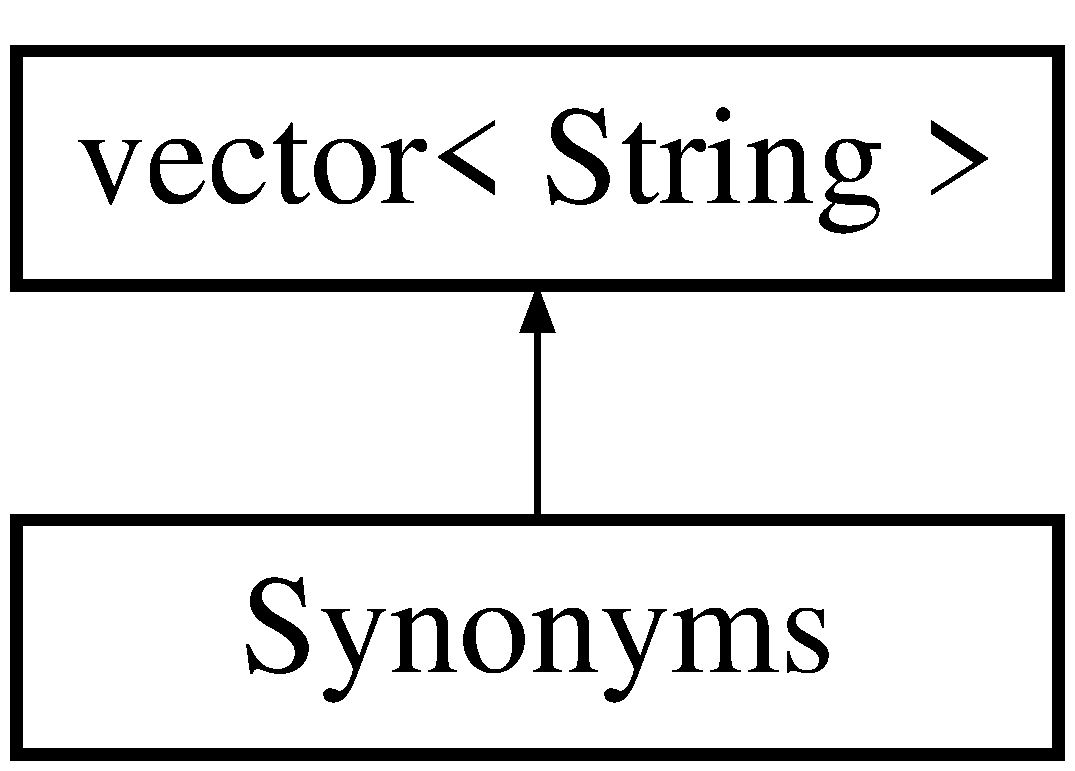
\includegraphics[height=2.000000cm]{classSynonyms}
\end{center}
\end{figure}
\subsection*{Public Member Functions}
\begin{DoxyCompactItemize}
\item 
\mbox{\hyperlink{classSynonyms_ac3bc326580cfe3de1bab88d71e5dcaed}{Synonyms}} (const \mbox{\hyperlink{classString}{String}} word)
\begin{DoxyCompactList}\small\item\em Default constructor\+: creates an empty list and adds. \end{DoxyCompactList}\item 
\mbox{\Hypertarget{classSynonyms_adfe3753a58fa0eb1d4b2409351f040c4}\label{classSynonyms_adfe3753a58fa0eb1d4b2409351f040c4}} 
\mbox{\hyperlink{classSynonyms_adfe3753a58fa0eb1d4b2409351f040c4}{Synonyms}} (const vector$<$ \mbox{\hyperlink{classString}{String}} $>$ \&\+\_\+\+\_\+x)
\begin{DoxyCompactList}\small\item\em Constructor\+: creates list from a vector of words. \end{DoxyCompactList}\item 
\mbox{\hyperlink{classString}{String}} \mbox{\hyperlink{classSynonyms_abe26e020a2d097a225bc0527253d9c63}{as\+Regex}} ()
\item 
bool \mbox{\hyperlink{classSynonyms_a36ffe85c896f9293626deab7d6517b51}{has\+Word}} (\mbox{\hyperlink{classString}{String}} word)
\end{DoxyCompactItemize}
\subsection*{Friends}
\begin{DoxyCompactItemize}
\item 
\mbox{\Hypertarget{classSynonyms_a6ee5cdecaeba3d88a245f0b9db2d2758}\label{classSynonyms_a6ee5cdecaeba3d88a245f0b9db2d2758}} 
ostream \& {\bfseries operator$<$$<$} (ostream \&os, const \mbox{\hyperlink{classSynonyms}{Synonyms}} \&synonyms)
\end{DoxyCompactItemize}


\subsection{Detailed Description}
List of synonyms. 

\subsection{Constructor \& Destructor Documentation}
\mbox{\Hypertarget{classSynonyms_ac3bc326580cfe3de1bab88d71e5dcaed}\label{classSynonyms_ac3bc326580cfe3de1bab88d71e5dcaed}} 
\index{Synonyms@{Synonyms}!Synonyms@{Synonyms}}
\index{Synonyms@{Synonyms}!Synonyms@{Synonyms}}
\subsubsection{\texorpdfstring{Synonyms()}{Synonyms()}}
{\footnotesize\ttfamily Synonyms\+::\+Synonyms (\begin{DoxyParamCaption}\item[{const \mbox{\hyperlink{classString}{String}}}]{word }\end{DoxyParamCaption})}



Default constructor\+: creates an empty list and adds. 


\begin{DoxyParams}{Parameters}
{\em word} & into the list. \\
\hline
\end{DoxyParams}


\subsection{Member Function Documentation}
\mbox{\Hypertarget{classSynonyms_abe26e020a2d097a225bc0527253d9c63}\label{classSynonyms_abe26e020a2d097a225bc0527253d9c63}} 
\index{Synonyms@{Synonyms}!as\+Regex@{as\+Regex}}
\index{as\+Regex@{as\+Regex}!Synonyms@{Synonyms}}
\subsubsection{\texorpdfstring{as\+Regex()}{asRegex()}}
{\footnotesize\ttfamily \mbox{\hyperlink{classString}{String}} Synonyms\+::as\+Regex (\begin{DoxyParamCaption}{ }\end{DoxyParamCaption})}

Translates synonyms list into a R\+E\+G\+EX group expression. \begin{DoxyReturn}{Returns}
words list separated by \char`\"{}$\vert$\char`\"{} 
\end{DoxyReturn}
\mbox{\Hypertarget{classSynonyms_a36ffe85c896f9293626deab7d6517b51}\label{classSynonyms_a36ffe85c896f9293626deab7d6517b51}} 
\index{Synonyms@{Synonyms}!has\+Word@{has\+Word}}
\index{has\+Word@{has\+Word}!Synonyms@{Synonyms}}
\subsubsection{\texorpdfstring{has\+Word()}{hasWord()}}
{\footnotesize\ttfamily bool Synonyms\+::has\+Word (\begin{DoxyParamCaption}\item[{\mbox{\hyperlink{classString}{String}}}]{word }\end{DoxyParamCaption})}

Searches for a word in synonyms list. 
\begin{DoxyParams}{Parameters}
{\em word} & \\
\hline
\end{DoxyParams}
\begin{DoxyReturn}{Returns}
True if word in list, False otherwise 
\end{DoxyReturn}


The documentation for this class was generated from the following files\+:\begin{DoxyCompactItemize}
\item 
src/\+Agent/\+E\+L\+I\+Z\+A/Synonyms.\+h\item 
src/\+Agent/\+E\+L\+I\+Z\+A/Synonyms.\+cpp\end{DoxyCompactItemize}

\hypertarget{classThesaurus}{}\section{Thesaurus Class Reference}
\label{classThesaurus}\index{Thesaurus@{Thesaurus}}


List of \mbox{\hyperlink{classSynonyms}{Synonyms}} objects.  




{\ttfamily \#include $<$Thesaurus.\+h$>$}

Inheritance diagram for Thesaurus\+:\begin{figure}[H]
\begin{center}
\leavevmode
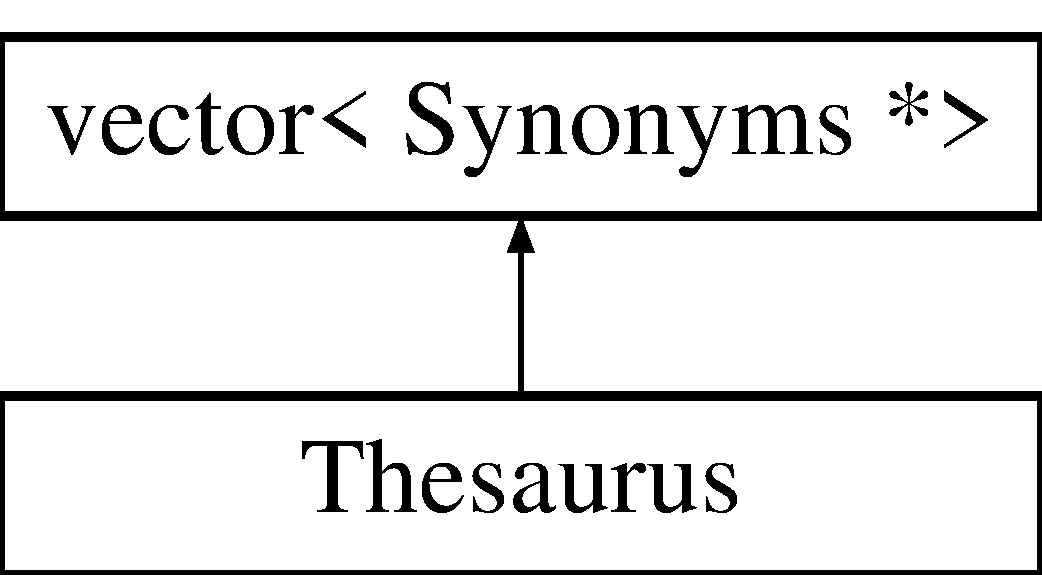
\includegraphics[height=2.000000cm]{classThesaurus}
\end{center}
\end{figure}
\subsection*{Public Member Functions}
\begin{DoxyCompactItemize}
\item 
\mbox{\hyperlink{classSynonyms}{Synonyms}} $\ast$ \mbox{\hyperlink{classThesaurus_ab21a3efabe41ac712734cbcc6d7d4414}{find\+Synonyms}} (\mbox{\hyperlink{classString}{String}} word)
\end{DoxyCompactItemize}
\subsection*{Friends}
\begin{DoxyCompactItemize}
\item 
\mbox{\Hypertarget{classThesaurus_a8cd7efb378b35ca92645c98c8164314b}\label{classThesaurus_a8cd7efb378b35ca92645c98c8164314b}} 
ostream \& {\bfseries operator$<$$<$} (ostream \&os, const \mbox{\hyperlink{classThesaurus}{Thesaurus}} \&thesaurus)
\end{DoxyCompactItemize}


\subsection{Detailed Description}
List of \mbox{\hyperlink{classSynonyms}{Synonyms}} objects. 

\subsection{Member Function Documentation}
\mbox{\Hypertarget{classThesaurus_ab21a3efabe41ac712734cbcc6d7d4414}\label{classThesaurus_ab21a3efabe41ac712734cbcc6d7d4414}} 
\index{Thesaurus@{Thesaurus}!find\+Synonyms@{find\+Synonyms}}
\index{find\+Synonyms@{find\+Synonyms}!Thesaurus@{Thesaurus}}
\subsubsection{\texorpdfstring{find\+Synonyms()}{findSynonyms()}}
{\footnotesize\ttfamily \mbox{\hyperlink{classSynonyms}{Synonyms}} $\ast$ Thesaurus\+::find\+Synonyms (\begin{DoxyParamCaption}\item[{\mbox{\hyperlink{classString}{String}}}]{word }\end{DoxyParamCaption})}

Finds \mbox{\hyperlink{classSynonyms}{Synonyms}} object containing a given word. Calls \mbox{\hyperlink{classSynonyms_a36ffe85c896f9293626deab7d6517b51}{Synonyms\+::has\+Word}}~\newline
If none found, returns a new synonyms list containing only the given word. 
\begin{DoxyParams}{Parameters}
{\em word} & \\
\hline
\end{DoxyParams}
\begin{DoxyReturn}{Returns}
pointer to synonyms object containing word 
\end{DoxyReturn}


The documentation for this class was generated from the following files\+:\begin{DoxyCompactItemize}
\item 
src/\+Agent/\+E\+L\+I\+Z\+A/Thesaurus.\+h\item 
src/\+Agent/\+E\+L\+I\+Z\+A/Thesaurus.\+cpp\end{DoxyCompactItemize}

\hypertarget{classWebClient}{}\section{Web\+Client Class Reference}
\label{classWebClient}\index{Web\+Client@{Web\+Client}}


{\ttfamily \#include $<$Web\+Client.\+h$>$}

Inheritance diagram for Web\+Client\+:\begin{figure}[H]
\begin{center}
\leavevmode
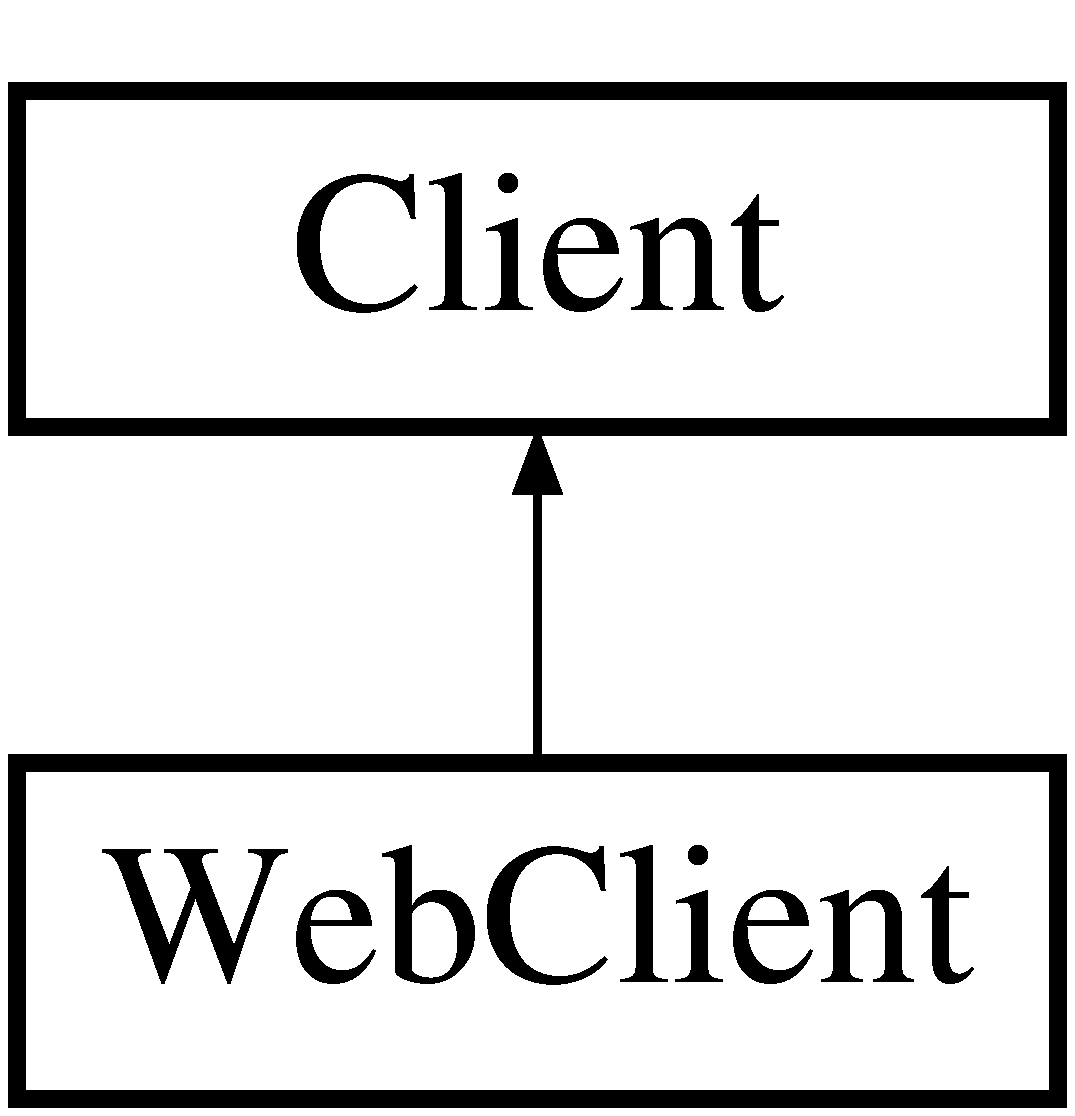
\includegraphics[height=2.000000cm]{classWebClient}
\end{center}
\end{figure}
\subsection*{Static Public Member Functions}
\begin{DoxyCompactItemize}
\item 
static void \mbox{\hyperlink{classWebClient_a6a78982b8b198331bddf50ec02b6bc8c}{send}} ()
\end{DoxyCompactItemize}


\subsection{Detailed Description}
Project Chat\+Bot 

\subsection{Member Function Documentation}
\mbox{\Hypertarget{classWebClient_a6a78982b8b198331bddf50ec02b6bc8c}\label{classWebClient_a6a78982b8b198331bddf50ec02b6bc8c}} 
\index{Web\+Client@{Web\+Client}!send@{send}}
\index{send@{send}!Web\+Client@{Web\+Client}}
\subsubsection{\texorpdfstring{send()}{send()}}
{\footnotesize\ttfamily void Web\+Client\+::send (\begin{DoxyParamCaption}{ }\end{DoxyParamCaption})\hspace{0.3cm}{\ttfamily [static]}}

Project Chat\+Bot \mbox{\hyperlink{classWebClient}{Web\+Client}} implementation 

The documentation for this class was generated from the following files\+:\begin{DoxyCompactItemize}
\item 
src/\+Client/\+Web/Web\+Client.\+h\item 
src/\+Client/\+Web/Web\+Client.\+cpp\end{DoxyCompactItemize}

\chapter{File Documentation}
\hypertarget{Action_8h}{}\section{src/\+Agent/\+Knowledge\+Base/\+Action.h File Reference}
\label{Action_8h}\index{src/\+Agent/\+Knowledge\+Base/\+Action.\+h@{src/\+Agent/\+Knowledge\+Base/\+Action.\+h}}
{\ttfamily \#include \char`\"{}Sentence.\+h\char`\"{}}\newline
{\ttfamily \#include \char`\"{}K\+B.\+h\char`\"{}}\newline
\subsection*{Classes}
\begin{DoxyCompactItemize}
\item 
class \mbox{\hyperlink{classAction}{Action}}
\begin{DoxyCompactList}\small\item\em Represents an action undertaken by the knowledge-\/based agent. \end{DoxyCompactList}\end{DoxyCompactItemize}


\subsection{Detailed Description}
\begin{DoxyAuthor}{Author}
Ergi, Rand, Yuge 
\end{DoxyAuthor}

\hypertarget{Analyser_8h}{}\section{src/\+Agent/\+Knowledge\+Base/\+Analyser.h File Reference}
\label{Analyser_8h}\index{src/\+Agent/\+Knowledge\+Base/\+Analyser.\+h@{src/\+Agent/\+Knowledge\+Base/\+Analyser.\+h}}
{\ttfamily \#include \char`\"{}../\+Parser.\+h\char`\"{}}\newline
\subsection*{Classes}
\begin{DoxyCompactItemize}
\item 
class \mbox{\hyperlink{classAnalyser}{Analyser}}
\begin{DoxyCompactList}\small\item\em The analyser is responsible for the different parsing jobs that are used by the agent. \end{DoxyCompactList}\end{DoxyCompactItemize}


\subsection{Detailed Description}
\begin{DoxyAuthor}{Author}
Ergi, Rand, Yuge 
\end{DoxyAuthor}

\hypertarget{FLAnalyser_8h}{}\section{src/\+Agent/\+Knowledge\+Base/\+F\+L\+Analyser.h File Reference}
\label{FLAnalyser_8h}\index{src/\+Agent/\+Knowledge\+Base/\+F\+L\+Analyser.\+h@{src/\+Agent/\+Knowledge\+Base/\+F\+L\+Analyser.\+h}}
{\ttfamily \#include $<$vector$>$}\newline
{\ttfamily \#include \char`\"{}Analyser.\+h\char`\"{}}\newline
{\ttfamily \#include \char`\"{}Sentence.\+h\char`\"{}}\newline
\subsection*{Classes}
\begin{DoxyCompactItemize}
\item 
class \mbox{\hyperlink{classFLAnalyser}{F\+L\+Analyser}}
\begin{DoxyCompactList}\small\item\em This class uses the parse tree generated by the parser and translates it into a formal language (a small set of the English language in this case) \end{DoxyCompactList}\end{DoxyCompactItemize}


\subsection{Detailed Description}
\begin{DoxyAuthor}{Author}
Ergi, Rand, Yuge 
\end{DoxyAuthor}

\hypertarget{KB_8h}{}\section{src/\+Agent/\+Knowledge\+Base/\+KB.h File Reference}
\label{KB_8h}\index{src/\+Agent/\+Knowledge\+Base/\+K\+B.\+h@{src/\+Agent/\+Knowledge\+Base/\+K\+B.\+h}}
{\ttfamily \#include $<$vector$>$}\newline
{\ttfamily \#include \char`\"{}Sentence.\+h\char`\"{}}\newline
{\ttfamily \#include \char`\"{}K\+B\+Analyser.\+h\char`\"{}}\newline
{\ttfamily \#include \char`\"{}Rule.\+h\char`\"{}}\newline
\subsection*{Classes}
\begin{DoxyCompactItemize}
\item 
class \mbox{\hyperlink{classKB}{KB}}
\begin{DoxyCompactList}\small\item\em This class represents our knowledge base. \end{DoxyCompactList}\end{DoxyCompactItemize}


\subsection{Detailed Description}
\begin{DoxyAuthor}{Author}
Ergi, Rand , Yuge 
\end{DoxyAuthor}

\hypertarget{KBAgent_8h}{}\section{src/\+Agent/\+Knowledge\+Base/\+K\+B\+Agent.h File Reference}
\label{KBAgent_8h}\index{src/\+Agent/\+Knowledge\+Base/\+K\+B\+Agent.\+h@{src/\+Agent/\+Knowledge\+Base/\+K\+B\+Agent.\+h}}
{\ttfamily \#include \char`\"{}../\+Agent.\+h\char`\"{}}\newline
{\ttfamily \#include \char`\"{}Percept.\+h\char`\"{}}\newline
{\ttfamily \#include \char`\"{}Action.\+h\char`\"{}}\newline
{\ttfamily \#include \char`\"{}K\+B.\+h\char`\"{}}\newline


\subsection{Detailed Description}
\begin{DoxyAuthor}{Author}
Ergi, Rand, Yuge 
\end{DoxyAuthor}

\hypertarget{KBAnalyser_8h}{}\section{src/\+Agent/\+Knowledge\+Base/\+K\+B\+Analyser.h File Reference}
\label{KBAnalyser_8h}\index{src/\+Agent/\+Knowledge\+Base/\+K\+B\+Analyser.\+h@{src/\+Agent/\+Knowledge\+Base/\+K\+B\+Analyser.\+h}}
{\ttfamily \#include \char`\"{}Analyser.\+h\char`\"{}}\newline
{\ttfamily \#include \char`\"{}../\+Parser.\+h\char`\"{}}\newline
\subsection*{Classes}
\begin{DoxyCompactItemize}
\item 
class \mbox{\hyperlink{classKBAnalyser}{K\+B\+Analyser}}
\begin{DoxyCompactList}\small\item\em This class represents the analyser responsible for parsing the First Order Logic language. \end{DoxyCompactList}\end{DoxyCompactItemize}


\subsection{Detailed Description}
\begin{DoxyAuthor}{Author}
Ergi, Rand, Yuge 
\end{DoxyAuthor}

\hypertarget{Percept_8h}{}\section{src/\+Agent/\+Knowledge\+Base/\+Percept.h File Reference}
\label{Percept_8h}\index{src/\+Agent/\+Knowledge\+Base/\+Percept.\+h@{src/\+Agent/\+Knowledge\+Base/\+Percept.\+h}}
{\ttfamily \#include \char`\"{}Sentence.\+h\char`\"{}}\newline
{\ttfamily \#include $<$vector$>$}\newline
{\ttfamily \#include $<$iostream$>$}\newline
\subsection*{Classes}
\begin{DoxyCompactItemize}
\item 
class \mbox{\hyperlink{classPercept}{Percept}}
\begin{DoxyCompactList}\small\item\em This class represents a perception received by the agent (which is of an exclusive text form in our case). \end{DoxyCompactList}\end{DoxyCompactItemize}


\subsection{Detailed Description}
\begin{DoxyAuthor}{Author}
Ergi, Rand, yuge 
\end{DoxyAuthor}

\hypertarget{Rule_8h}{}\section{src/\+Agent/\+Knowledge\+Base/\+Rule.h File Reference}
\label{Rule_8h}\index{src/\+Agent/\+Knowledge\+Base/\+Rule.\+h@{src/\+Agent/\+Knowledge\+Base/\+Rule.\+h}}
{\ttfamily \#include \char`\"{}Sentence.\+h\char`\"{}}\newline
{\ttfamily \#include $<$vector$>$}\newline
{\ttfamily \#include $<$iostream$>$}\newline


\subsection{Detailed Description}
\begin{DoxyAuthor}{Author}
Ergi, Rand, Yuge 
\end{DoxyAuthor}

\hypertarget{Sentence_8h}{}\section{src/\+Agent/\+Knowledge\+Base/\+Sentence.h File Reference}
\label{Sentence_8h}\index{src/\+Agent/\+Knowledge\+Base/\+Sentence.\+h@{src/\+Agent/\+Knowledge\+Base/\+Sentence.\+h}}
\subsection*{Classes}
\begin{DoxyCompactItemize}
\item 
class \mbox{\hyperlink{classSentence}{Sentence}}
\begin{DoxyCompactList}\small\item\em Class representing a sentence. \end{DoxyCompactList}\end{DoxyCompactItemize}


\subsection{Detailed Description}
\begin{DoxyAuthor}{Author}
Ergi, Rand, Yuge 
\end{DoxyAuthor}

%--- End generated contents ---

% Index
\backmatter
\newpage
\phantomsection
\clearemptydoublepage
\addcontentsline{toc}{chapter}{Index}
\printindex

\end{document}
